\documentclass[11pt,peerreview]{IEEEtran}

%\usepackage[backend=bibtex]{biblatex}
%ARABIC SECTIONS
\renewcommand\thesection{\arabic{section}}
\renewcommand\thesubsection{\thesection.\arabic{subsection}}
\renewcommand\thesubsubsection{\thesubsection.\arabic{subsubsection}}

\renewcommand\thesectiondis{\arabic{section}}
\renewcommand\thesubsectiondis{\thesectiondis.\arabic{subsection}}
\renewcommand\thesubsubsectiondis{\thesubsectiondis.\arabic{subsubsection}}

\usepackage[version=3]{acro}
\usepackage{caption}
\raggedbottom
\usepackage{mathtools}
\usepackage{graphicx}
\usepackage{color}
\usepackage[margin=1in]{geometry}
\usepackage{amsfonts,amsmath,amssymb}
\usepackage[none]{hyphenat}
\usepackage[nottoc,notlot,notlof]{tocbibind}
\usepackage{fixltx2e}
\usepackage{siunitx}
\usepackage{longtable}
\usepackage{subfigure}
\usepackage{caption}
\usepackage{algorithm2e}

\sisetup{per-mode=symbol}
%Clikcable Links
\usepackage{hyperref}
\hypersetup{
    colorlinks,
    citecolor=black,
    filecolor=black,
    linkcolor=black,
    urlcolor=blue
} 

\usepackage{floatrow}
\floatsetup[table]{capposition=top}
\pagenumbering{Roman}
\setlength{\parskip}{1em}
\renewcommand{\baselinestretch}{1.5}

\DeclareAcronym{acm}{
  short = ACM ,
  long  = Association for Computing Machinery ,
}

\DeclareAcronym{gps}{
  short = GPS ,
  long  = Global Positioning System ,
}
\DeclareAcronym{io}{
  short = I/O ,
  long  = Input/Output ,
}

\DeclareAcronym{mqtt}{
  short = MQTT ,
  long  = Message Queuing Telemetry Transport  ,
}

\DeclareAcronym{coap}{
  short = CoAP ,
  long  = Constrained Application Protocol ,
}

\DeclareAcronym{can}{
  short = CAN ,
  long  = Control Area Network ,
}

\DeclareAcronym{ui}{
  short = UI ,
  long  = User Interface ,
}

\DeclareAcronym{dao}{
  short = DAO ,
  long  = Data Access Object ,
}

\DeclareAcronym{tcp}{
  short = TCP ,
  long  = Transfer Control Protocol ,
}

\DeclareAcronym{vps}{
  short = VPS ,
  long  = Virtual Private Server ,
}

\DeclareAcronym{uuid}{
  short = UUID ,
  long  = Universally Unique Identifier ,
}

\DeclareAcronym{uri}{
  short = URI ,
  long  = Uniform Resource Identifier ,
}

\DeclareAcronym{ip}{
  short = IP ,
  long  = internet protocol ,
}

\DeclareAcronym{ca}{
  short = CA ,
  long  = Certificate Authority ,
}

\DeclareAcronym{apk}{
  short = APK ,
  long  = Android Package ,
}

\DeclareAcronym{rest}{
  short = REST ,
  long  = Representational State Transfer
}

\DeclareAcronym{html}{
  short = HTML ,
  long  = HyperText Markup Language ,
}

\DeclareAcronym{css}{
  short = CSS ,
  long  = Cascading Style Sheets ,
}

\DeclareAcronym{ecu}{
  short = ECU ,
  long  = Electronic Control Unit ,
}

\DeclareAcronym{obd}{
  short = OBD ,
  long  = on-board diagnostic ,
}

\DeclareAcronym{sae}{
  short = SAE ,
  long  = Society of Automotive Engineers ,
}

\DeclareAcronym{ios}{
  short = iOS ,
  long  = iPhone Operating System ,
}

\DeclareAcronym{jvm}{
  short = JVM ,
  long  = Java Virtual Machine ,
}

\DeclareAcronym{rdbms}{
  short = RDBMS ,
  long  = Relational Database Management Systems ,
}

\DeclareAcronym{sql}{
  short = SQL ,
  long  = Structured Query Language ,
}

\DeclareAcronym{nosql}{
  short = NoSQL ,
  long  = Not only SQL ,
}

\DeclareAcronym{soc}{
  short = SoC ,
  long  = Separation of Concerns ,
}

\DeclareAcronym{ssl}{
  short = SSL ,
  long  = Secure Socket Layer ,
}

\DeclareAcronym{di}{
  short = DI ,
  long  = Dependency Injection ,
}

\DeclareAcronym{oop}{
  short = OOP ,
  long  = object-oriented programming ,
}

\DeclareAcronym{mvc}{
  short = MVC ,
  long  = Model-View-Controller ,
}

\DeclareAcronym{mvvm}{
  short = MVVM ,
  long  = Model-View-ViewModel ,
}

\DeclareAcronym{orm}{
  short = ORM ,
  long  = Object Relational Mapper ,
}

\DeclareAcronym{app}{
  short = app ,
  long  = application ,
}

\DeclareAcronym{tls}{
  short = TLS ,
  long  = Transport Layer Security ,
}

\DeclareAcronym{http}{
  short = HTTP ,
  long  = Hypertext Transfer Protocol ,
}

\DeclareAcronym{https}{
  short = HTTPS ,
  long  = Hypertext Transfer Protocol Secure ,
}

\DeclareAcronym{json}{
  short = JSON ,
  long  = JavaScript Object Notation ,
}

\DeclareAcronym{xml}{
  short = XML ,
  long  = Extensible Markup Language ,
}

\DeclareAcronym{uml}{
  short = UML ,
  long  = Unified Modelling Language ,
}

\DeclareAcronym{api}{
  short = API ,
  long  = Application Programming Interface ,
}

\DeclareAcronym{id}{
  short = ID ,
  long  = Identity ,
}

\acsetup{
    make-links ,
    pages / display = all ,
    pages / fill = {, },
    list / template = longtable ,
}

\usepackage{pdfpages}
\setlength{\parindent}{0em}
% Keywords command
\providecommand{\keywords}[1]
{
  \small	
  \textbf{\textit{Keywords---}} #1
}

\begin{document}

\begin{titlepage}

\includepdf[pages={1}, width=\paperwidth, height=\paperheight]{cover.pdf}
\end{titlepage}
%regular prerequisites for a document, contents, tables, figures
\begin{abstract}
\noindent Trucking companies require a means to track their employees, ensuring they perform their work as expected, and do so in a safe, legal manner.
Acceleration, altitude, location and speed are identified variables of interest to adequately determine trucking behavior.
This brings about the need for a real-time tracking system, logging these variables for each trucker in a fleet.\\

\noindent Dedicated, single-purpose boards with GPS and sensor capability offer a common solution.
Another solution is offered by making use of smartphones, for their multipurpose capabilities.
Managers may require their truckers to make use of other smartphone applications, potentially including stock-tracking and communication systems.
One smartphone could perform all of these activities if tracking was also handled by the device.
To this end, a software tracking solution is proposed making use of smartphone devices with built-in GPS and sensor capability.
The proposal entails the development of a smartphone application for continuous data logging, an input/output server for relaying data from the smartphones to a central data store, and a web application allowing managers to manage and view data from their truckers.
The main identified objective is to provide managers an interface to monitor the movement of their truckers.\\

\noindent Software design principles are utilized in the design and implementation of an Android application, asynchronous input/output server in C++ and a web application in C\# using the ASP.NET web framework.
Common design paradigms which aim to improve the modularity and scalability of software are implemented in the solution.
A simple algorithm is implemented for processing raw GPS data, determining the truckers activities which includes start/stop times and average acceleration, altitude, location and speed during trips.\\

\noindent The resulting implemented solution allows Android users to operate the application in the background while doing other tasks.
Managers using the web application are presented with a map interface highlighting trip paths, stopping points and times, and graphs showcasing percentile distributions of the logged variables.
The solution is tested on several Android devices, with reports accessed for correctness.
\\

\noindent Reliability concerns are noted, with the Android application dependent on the user making proper use of it.
Further software improvements are identified for improving the robustness of the solution up-time.
The proposed solution presents an interesting alternative for budget conscious managers, who require extra functionality in addition to just tracking.
\end{abstract}
\keywords{Acceleration, Altitude, Android, Global Positioning System, Software Design, Speed, Tracking}

\pagebreak

\tableofcontents
\pagebreak
\listoffigures
\listoftables
\pagebreak
\printacronyms
\pagebreak

\pagenumbering{arabic}
\setcounter{page}{1}

\section{Introduction}
\subsection{Purpose of document}
This report documents the contextualization of a problem surrounding the tracking of truckers.
The background and problem is considered, and possible solutions with objectives are identified, along with an expected outcome for the potential solution, requirements and scope definition.
The design and implementation of a solution are investigated.

\subsection{Background}
Due to the nature of the trucking industry, it is difficult for company owners to keep track of their employees.
Truckers carry out their shifts delivering important cargo to various locations over far distances.
As such, it is not practical for employers to track their whereabouts throughout their shifts.
This allows truckers the ability to behave undesirably while on the job.
Truckers who waste time taking unnecessarily long stops or detours waste company time and money.
In addition, some truckers may also be found breaking traffic laws without proper intervention.
Such employees are a liability to the reputation and profitability of their respective companies.

The ability to track truckers would provide a potential means to address this issue, by allowing employers to monitor their truckers' location, progress and behavior throughout their shifts.
The ability to produce an audit trail detailing the truckers whereabouts during their shifts would allow managers to ensure that work is adequately executed. Such an audit trail would comprise of:
\begin{itemize}
\item \textbf{\ac{gps} coordinates\\}
\ac{gps} tracking will allow employers to ensure that truckers are actually traveling to required locations, and doing so via the most effective routes. This also allows employers to ensure no unnecessary detours occur.
\item \textbf{Altitude\\}
An optional parameter which may be useful in some cases.
\item \textbf{Speed\\}
Examining the trucker's speed allows for managers to examine the effectiveness of cargo transportation, and to ensure that traffic laws are generally obeyed.
\item \textbf{Acceleration\\}
A potentially useful parameter which may be used for inferring any dangerous driving behavior. 
\end{itemize}

The ubiquitous nature of cheap, \ac{gps}-equipped smartphones provides a potential avenue for realizing such a solution at low cost.
In addition, country-wide continuous access to the internet allows for live tracking to be utilized. 

\subsection{Problem Statement}
A smartphone-powered tracking system must be implemented to be used by trucking companies for tracking and logging their trucker's \textbf{\ac{gps} coordinates, altitude, speed and acceleration}.

In addition, an online interface is required for storing, processing and displaying logged data pertaining to the trucker's location and behavior.

\subsection{Hypothesis}
An anticipated architecture, as depicted in figure \ref{fig:high_arch}, involves the development of a smartphone application capable of interfacing with internal or external sensors, and transferring sensor data through some \ac{io} server into a data store. \cite{bertocco1998client}
For the purposes of information presentation, it is proposed that a web server process and serve inferred information to a user via a web application.
\begin{figure}[H]
    \centering
    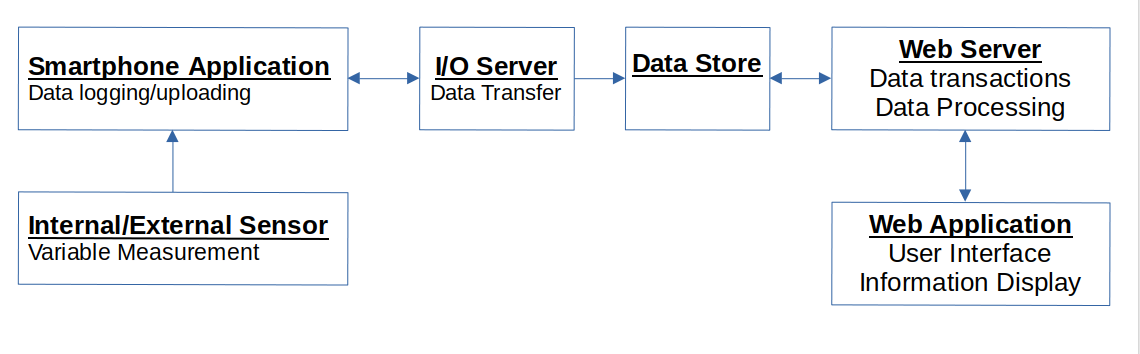
\includegraphics[scale=0.45]{high_arch.png}
    \caption{Proposed High Level Architecture}
    \label{fig:high_arch}
\end{figure}

\subsection{Project Objective}
\subsubsection{Primary Objective}
The primary objective in addressing the problem will be the development of detailed reports showcasing the trucker's whereabouts and behavior during their work shifts.

\subsection{Anticipated Benefits of Solution}
Managers will be able to ensure that their truckers conduct their work efficiently and responsibly.
They will then be able to adequately handle truckers who fail to perform as expected.

Managers may also be able to analyze trucker behavior to perform optimizations, potentially allowing for increased efficiency.

\subsection{Technical Requirements}
\subsubsection{Requirements}
\begin{enumerate}
\item \textbf{Smartphone Application}\\
    This will be a smartphone application used by the entities being tracked(i.e the truckers).
    \begin{enumerate}
        \item Trucker identification control must be implemented to ensure that logs sent to the server correspond to a unique trucker. It must not be possible for multiple truckers to assume the same or no identity.
        \item Every 2 minutes, sensor data capturing the \textbf{\ac{gps} coordinates, altitude, speed and acceleration} must be captured and stored internally on the android device. 
        Data capacity for one continuous week of storage must be possible, to account for connectivity issues.
        \item The application must be able to run in the background, allowing for multitasking.
        \item Sensor data must be uploaded to a central data store, either continuously or on request. This communication must be encrypted for security purposes.
    \end{enumerate}
\item \textbf{\ac{io} Server}\\
This server will facilitate the transfer of logged data from the Smartphone Application to a central data store, via an internet connection. 
    \begin{enumerate}
        \item As a dedicated transfer server, it must exhibit high performance, handling multiple requests from the multiple smartphone clients asynchronously.
        \item Trucker logs, received from smartphone clients, must be stored in a central database.
        \item Information about the trucking company must also be sent to the smartphone client.
    \end{enumerate}
\item \textbf{Data Store}\\
The data store will be efficient, fast and capable of storing large volumes of data.
It should also be capable of adequately interfacing with the \ac{io} server and the Web Server.
The web server is responsible for querying data from the data store, and serving requests to the web application.
\item \textbf{Web Server and Web Application}\\
The web server must implement back-end business logic and serve pages in the web application.
The web application acts as an interface for managers to add truckers and view tracking information about their fleets.
    \begin{enumerate}
        \item Multiple trucking managers must be able to log in and use the application.
        \item Managers must be able to add multiple truckers to their fleet, including trucker-specific information such as name, and vehicle number.
        \item Managers must be able to view detailed trip information for any adjustable time period. Log data must be processed to determine starting and arrival times for locations traveled to. Statistical information about acceleration and speed should be displayed, including averages, maximums and percentiles.
    \end{enumerate}
\end{enumerate}
\subsubsection{Scope Definition}
The scope of the problem considered will include
\begin{enumerate}
\item \textbf{Internal/External Sensor Interface}\\
The scope \textbf{does not} include the design of sensor circuitry meant to interface with the smartphone. Only configurations capable of interfacing with the smartphone are considered.
The smartphone app is not concerned with displaying user reports and statistics. That is left to the web application.
\item \textbf{Smartphone Application}\\
The smartphone application is purely responsible for logging the appropriate sensor data and transferring the sensor data on through the \ac{io} server.
Other measurable variables such as temperature, fuel and pressure are not considered.
\item \textbf{\ac{io} Server}\\
The \ac{io} server is purely responsible for facilitating the transfer of sensor data from the smartphone to the data store.
\item \textbf{Data Store}\\
    The data store element is purely concerned with the storage of logs, user identity information and providing an interface for the \ac{io} server to query and add records to the store.
    Existing data store providers will be considered.
\end{enumerate}

\subsection{Deliverables}
The deliverables will require the entire project to function, from the smartphone logging implementation, to the detailed reports available in the web application. 
\begin{itemize}
\item Smartphone Application and \ac{io} server
\item Web Application and web server
\end{itemize}

\subsection{Conclusion}
Basic contextualization of the problem has been performed.
Low level details, however, have not been considered.
Each aspect of the planned architecture may be realized in multiple ways on the low level.
Further research and a feasibility analysis are necessary for adequate low level design.

\pagebreak

\section{Literature Review}
This section tackles the investigation of components which make up the proposed high level system depicted in figure \ref{fig:hypothesis}.
There exists a variety of different tools available to realize each system.
With the hardware preexisting, most of the design exists in the software domain.
Various software tools and methodologies are considered.

\subsection{Sensors}
Effective data logging of acceleration, altitude, location and speed begin with the quality of measurements being made.
Smartphones alone provide a wealth of options.
However, external sensors available to the truck operators offer a variety of options.

\subsubsection{Internal Sensors}
Most smartphones come well-equipped with a wide variety of on-board sensors, such as \ac{gps} sensors, accelerometers, gyroscopes, magnetometers and ambient light sensors, among others \cite{majumder2019smartphone}.
As such, they are capable of inferring a wealth of information related to driving patterns.
This includes dangerous driving behavior, for which algorithms have been developed \cite{li2016dangerous}.

While not all smartphones provide a full suite of sensors, a combination of on-board sensors can be used to measure variables of interest.
\begin{itemize}
\item \textbf{Acceleration}\\
Raw accelerometers provide acceleration readings along 3 axes to encompass a three dimensional space.
Tilting or rotating the smartphone will change the axis on which an applied acceleration is detected.
This will happen often in smartphones which aren't securely mounted, or when traversing steep gradients.
The combined applied acceleration (or resultant acceleration $a_{res}$) can be found by combining the component in each direction, with
\begin{equation}\label{eq:acc}
\begin{split}
a_{res} = \sqrt{a_{x}^2 + a_{y}^2 + a_{z}^2},\\
\end{split}
\end{equation}
where $a_{x}, a_{y}, a_{z}$ denote the acceleration components on each axis.\cite{david2020halliday}

Gravity applies a constant acceleration as well, which is not of interest.
Filters that eliminate this constant gravity component can do so by means of highpass filtering, clearing the constant bias.
However, if this acceleration is sustained for several samples (as is often the case when driving), this momentarily constant acceleration is also filtered out.

The most effective means for determining acceleration excluding gravity is to use a combination of sensors in a strategy usually termed \textit{sensor fusion}.\cite{sasiadek2002sensor}
This method makes additional use of magnetometers and gyroscopes to isolate and remove the gravity component.
An Android \ac{api} abstraction makes use of sensor fusion implementing a so-called \textit{linear accelerometer}, which allows for acceleration readings which exclude the influence of gravity.

\item \textbf{\Ac{gps} Location}\\
\Ac{gps} receivers are typically available in most modern smartphones.
They determine the user's \ac{gps} coordinates, which reveals their location.

\item \textbf{Speed}\\
Devices with \ac{gps} capabilities can infer speed using location-time differences.

\item \textbf{Altitude}\\
\Ac{gps} capable devices also supply altitude information.
\end{itemize}

Battery life preservation and reduced performance are often concerns when running computationally heavy daemons (background operating system processes).
Recent efforts in the development and standardization of new, lightweight sensor-probing protocols have been investigated.
Namely, \ac{mqtt} and \ac{coap}, which are targeted at achieving lightweight, low-power performance \cite{de2013comparison}.

\subsubsection{External Sensors}
The most practical means of utilizing sensors external to the smartphone may be realized through the use of in-vehicle sensors. 
The \ac{can} bus protocol is a centralized multiplex communication bus standard utilized in many modern vehicles, originally in an attempt to save on copper. 
The protocol allows for broadcast communication between various \ac{ecu}'s within a vehicle, all centrally connected to one bus.
A priority-based scheme is utilized to ensure the most important units transmit their data packets first, while lower priority units are delayed until a later time when transmission may be uninterrupted. Each packet contains an identifier designating what information is being transmitted, such as wheel speed, temperature, etc.
\cite{van2011canauth}

Assuming that the vehicle has an \ac{obd} connector, communication with a smartphone requires some form of interfacing circuitry.
Wireless \ac{can}-to-smartphone interfaces can be most-practically realized via \ac{can}-bus-to-Bluetooth implementations.
Such an interface will allow for the smartphone to probe sensor data via the vehicle's \ac{can} bus \cite{campolo2012smartcar} \cite{walter2013smartphone}.
The \ac{sae} defines the J1939 standard for \ac{can}-bus communication in the use of heavy-duty vehicles \cite{stepper1993j1939}, which would be appropriate for the solution.

\subsection{Software Architecture}
Effective software architecture and design patterns are necessary for writing dynamic, modifiable and modular software.

\subsubsection{\ac{soc} and SOLID principles}
\Ac{soc} addresses the need for software to be decomposed into different modular units.
Each unit focuses on one main concern, such as data access, authentication, business logic and view rendering.
Mixing multiple concerns within one unit leads to code which is less reusable and more difficult to modify.
\cite{gamageseparation}

The 'SOLID' acronym defines a set of guidelines for software design, in \ac{oop}.
\begin{enumerate}
\item \textbf{Single Responsibility Principle}\\
Classes should have single responsibilities. 
To achieve this, each responsibility must be implemented in a unique class.
\item \textbf{Open/Close Principle}\\
Software components such as classes, modules and functions should be open for extension, but closed for modification.
That is, classes implementing a modifiable functionality should be extended with interfaces instead of modifying code in the class.
\item \textbf{Liskov substitution Principle}\\
Objects should be replaceable with derived sub-types without affecting the correctness of the program.
\item \textbf{Interface Segregation Principle}\\
It is better to implement many client-specific interfaces instead of one general-purpose interface.
This ensures the interface being implemented only does the minimal that is required.
\item \textbf{Dependency Inversion Principle}\\
Where possible, it is better to depend on implementable abstractions instead of concretely defined objects.
This can be realized by depending on implementable interfaces instead of base classes.
This allows classes to be less tightly-bound to a base class, allowing for more modular code.
\end{enumerate}
\cite{chebanyuk2016approach}

\subsubsection{\Ac{di}}
Often classes require instances of other objects (or dependencies) to perform certain functions.
It is wasteful to re-instantiate these objects especially if they are used by other classes.
\Ac{di} provides a means to \textit{inject} an instance of a helper object into a class without explicitly recreating the dependency.
\cite{kocsis2017dependency}

Objects which exist for the lifetime of the application are known as singletons, and the use of singletons is often facilitated with \ac{di}.

\subsection{Smartphone Application}
The smartphone application is responsible for extracting the acceleration, altitude, location and speed data from the sensors and relaying this information to the data store.
Certain platform and development design decisions are investigated.

\subsubsection{Platform Considerations}
The two major mobile operating systems are Android (approximately 72.8 \% market share) and \ac{ios} (approximately 27.4 \% market share) \cite{statcountermaketshare}.
Android's high market share makes it an attractive option as a target platform for the Smartphone application component of the system.

\subsubsection{Development Technologies}
Native Android development officially supports the Java, Kotlin, C and C++ programming languages.
Kotlin, which compiles on the \ac{jvm}, has been pushed by Google as their suggested language for app development.
Kotlin aims to reduce the verbosity of traditional Java (which was the standard language used for app development), thereby reducing the prevalence of "bad coding practices." \cite{flauzino2018you}
It is noted that Java may still be preferable for programmers with prior Java experience, or in cases where more verbosity is preferred.
A native C/C++ tool-chain offers finer control of system hardware for potential performance boosts \cite{kwan2012google}.

Cross-platform development presents a popular option for developing applications for both major platforms.
Several development frameworks such as Xamarin, Flutter and Apache Cordova allow for cross-platform development, among others.
However, cross-platform development does impose potentially reduced performance, according to \cite{biorn2020empirical}.
In an ecosystem where hardware used by truck drivers has potential to be slower, cross-platform development is undesirable.

\subsubsection{Android - \Ac{mvvm} Design Pattern}
Figure \ref{fig:mvvm_layout} depicts the \ac{mvvm} architecture used in a typical android context.
The view (typically activities or fragments in Android) represents the actual rendered output visible to the user.
Data displayed by the view is accessed by the view model.
The separation of views and view models is necessary for Android applications due to the temporary nature of views.
That is, data stored purely in the view component is lost upon re-rendering of the view, while view models hold onto data for longer.\cite{noauthor_guide_nodate}

The repository singleton acts as a central holder of application data, which is then accessed by the multiple views. It also interacts with \ac{io} resources such as web resources and database access. Views request data through the repository, and as such shouldn't have direct handles to database connections. \cite{noauthor_guide_nodate}

\begin{figure}
\centering
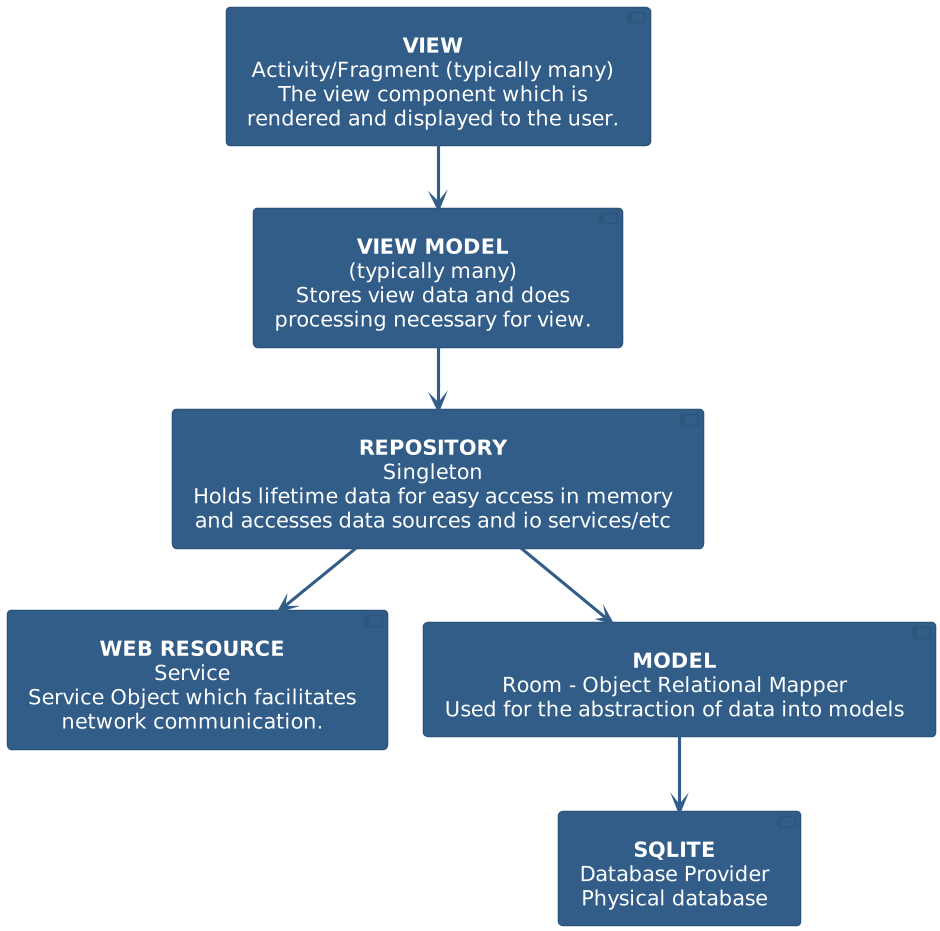
\includegraphics[scale=0.4]{../diag/mvvm_layout.png}
\caption{Android - \Ac{mvvm} Architecture}
\label{fig:mvvm_layout}
\end{figure}

\subsubsection{Android - \ac{di} with Hilt}
Hilt is an android library used for easily implementing \ac{di}.
It has support for common android components.
\cite{noauthor_dependency_nodate}

\subsubsection{Android - Running continuously in the background}
Tracking \ac{app}s need to run continuously, without forcing the user to keep the \ac{app} view components open.
This can be achieved by implementing the tracking component as a \textit{foreground service}.
In this way, the component runs continuously while allowing the user to use other applications.

Users must also be notified of continuously running services for clarity.
It is therefore required display notifications about the service.
\cite{noauthor_foreground_nodate}

\subsubsection{Android - SQLite database with the Room \ac{orm}}
The Room \ac{orm} library provides a neat database abstraction layer over SQLite useful for modeling data.
SQLite is preferable for android due to its lightweight nature.
\cite{noauthor_save_nodate}

The storage capacity of SQLite is basically unlimited.
Storage capacity is, however, limited to the storage capability of the smartphone running the application.
This makes the use of external storage desirable.

\subsection{\ac{io} Server}
The \ac{io} server is required for relaying logged data from the smartphone application to the central data store. It must be many clients quickly and efficiently.
This server plays a typical server role; In that it must await requests from clients attempting to establish connection for transmitting data.

Implementations for realizing such a server are possible in many programming languages, and almost all top popular programming languages. 
Generally, for performance-critical applications, C and/or C++ are considered most appropriate. \cite{ogala2020comparative}

\subsubsection{Asynchronous \Ac{io}}
Servers (and many other application) are required to perform relatively slow operations; that is communicating over networks and writing to disk.
Implementing such functionality synchronously (using blocking calls) leaves functions essentially waiting for data streams to be read, transmitted and written to disk.
This is slow and incapable of handling multiple simultaneous connections.

Asynchronous \ac{io} operations enables other processing to continue before a slow \ac{io} operation has completed.
This is essential for servers which handle many simultaneous connections.
A popular C++ library, \textit{asio} provides asynchronous \ac{io} functionality.
\cite{anggoro2015boost}

\subsection{Database Considerations}
\ac{rdbms}s are commonly used in for data handling.
Typically, for unnormalized complex data, conventional \ac{sql} \ac{rdbms}s prove inefficient at scale, due to the tendency of modern data catalogues lacking in structure.
In addition, relational databases also start to exhibit slower lookup times for immensely large data sets.
The solution to this comes in the form of \ac{nosql} database systems, which are scaleable, efficient and capable for storing large volumes of unnormalized data. \cite{gupta2017nosql} \cite{qader2018comparative} \cite{ongo2018hybrid}

However, due to the completely uniform structure of the data being stored, an \ac{rdbms} would suffice.
Numerous high quality \ac{rdbms}s, such as MySQL, Microsoft SQL, PostgreSQL, and Oracle Database are available, among others. All options offer relatively efficient performance.
\cite{truskowski2020comparison}

A lightweight caching database is necessary on the client-side for the momentary storage of data which has yet to be transmitted to the server. To this end, SQLite offers a popular solution for smartphone applications \cite{bhosale2015sqlite}.

\subsection{Web Application}
The web application will be used by managers to display daily reports highlighting their truckers' behavior throughout their shifts.

The web application may be easily realized by utilizing pre-existing web frameworks, such as Microsoft's ASP.NET Core and Oracle's Java Enterprise Edition (with comparable performance) \cite{kronis2018performance}.

\subsubsection{\Ac{mvc} design pattern for web applications}
\begin{figure}
\centering
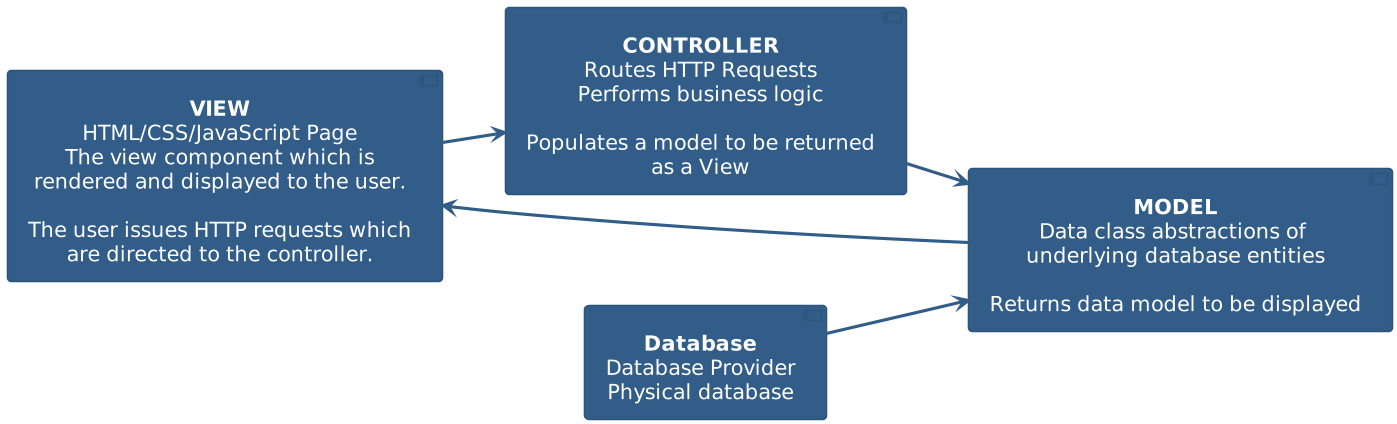
\includegraphics[width=6in]{../diag/mvc_layout.png}
\caption{Web Design Pattern - \ac{mvc}}
\label{fig:mvc_layout}
\end{figure}

A relatively popular design pattern in web development is the \ac{mvc} architecture.
As seen in figure \ref{fig:mvc_layout}, \ac{mvc} attempts to achieve \ac{soc} by separating logic required for viewing, routing and data into separate components.

\subsection{Secure communication with \ac{ssl}}
The use of secure communication over the internet is a modern-day standard.
And due to sensitive location data being transmitted, it is necessary to ensure that logs are adequately encrypted.

The \ac{ssl} protocol is a de facto standard for encrypted communication on the internet.
It makes use of cryptography as a means for clients to verify that communication is occurring with a trusted source.
\Ac{ssl} itself is deprecated, and the current standard for encryption is \ac{tls}.
However, it is common to refer to refer to these related technologies interchangeably, when \ac{tls} is the protocol actually in use. \cite{hickman1995ssl}

\subsection{Serialization and communication protocols}
Facilitating communication between two devices requires both devices to use the same protocol.
Regardless of this protocol, it is necessary for communication to be encrypted, therefore making use of \ac{ssl}.

\subsubsection{\Ac{https}}
\Ac{https} implements the de facto \Ac{http} protocol over the encrypted \ac{ssl} protocol.
\Ac{http} is an application layer protocol which makes use of standard headers carrying a payload under formalized request types, of which \textit{GET} and \textit{POST} are common.
\Ac{https} is commonly used for web services and websites.
\cite{fielding1999hypertext}.

\subsubsection{\Ac{json} and \Ac{xml}}
Serialization offers a means of converting runtime software objects into a byte stream format which can be transferred over the network. This is necessary for most inter-device communication.

\Ac{xml} is a strongly-typed text protocol which can be used for serialization.
It follows a tight tagging schema.

\Ac{json} is a fast and simple text protocol for serializing objects carrying data.
Support for arrays makes \ac{json} reliable for the transmission of many logs.
\cite{nurseitov2009comparison}

\pagebreak

\section{Design}
This section considers the context in which the problem exists and the design of each system and subsystem necessary to visualize and realize a possible solution to solve the problem.

The nature of the system exists primarily in the software domain.
As such, a suitable design architecture is postulated by the C4 model.
This model breaks down the system architecture into different layers of complexity, from a generic high-level system overview down to low-level software abstractions.\cite{vazquez2020c4}

Low-level abstractions are realized with \ac{uml} diagrams. \Ac{uml} diagrams detail the members and methods belonging to classes, and the relationships between those classes in an object-oriented codebase. \cite{petre2013uml}

\subsection{System context and base requirements }
Figure \ref{fig:system_context} depicts the system context in the problem domain.
Project specifications have identified two parties expected to utilize the system - truck drivers and fleet managers.
Identified requirements on the solution dictate that truck drivers will use an android application to log data on the system.
In addition, fleet managers must view the logged data and manipulate their fleets via a web application running in a browser.

\begin{figure}[H]
\centering
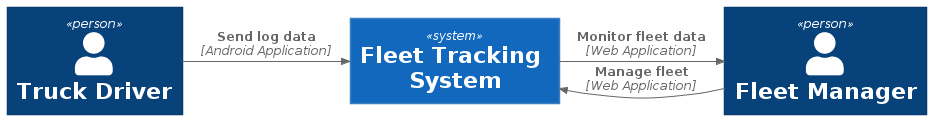
\includegraphics[width=6in]{../diag/system_context.png}
\caption{System Context Diagram}
\label{fig:system_context}
\end{figure}

\begin{figure}
\centering
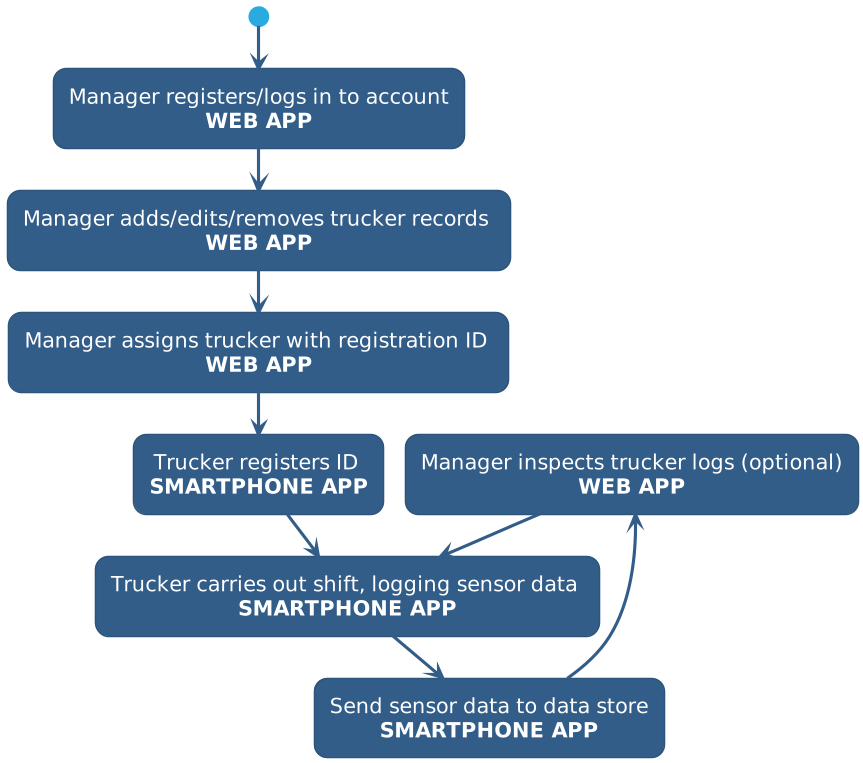
\includegraphics[scale=0.40]{../diag/high_level_activity.png}
\caption{System Lifecycle - High Level}
\label{fig:high_level_activity}
\end{figure}

The high-level life cycle view of the fleet-tracking system design is depicted in figure \ref{fig:high_level_activity}.
This life cycle view gives a broad indication of how the system is expected to work for a user.
Only front-end components of the system are considered to clarify exactly how users will interact with the system.

Managers are required to perform initial configuration, including adding trucker identity records to a data store.
After this, truckers may connect to the system and perform their work while allowing their smartphone applications to track the required sensor data. 
This data is then relayed to the system, in which managers may analyze and inspect data logs.

\subsection{Contained subsystems and choice of technologies}
The second level of the C4 model identifies the choice of technologies to be utilized to realize the fleet tracking system.
The fleet-tracking system is divided into mostly-independent containers, as depicted in figure \ref{fig:container}.
Each container is a standalone process which makes calls to other processes in the system.
The main choice of software tools are identified for each container.

Truckers will make use of an android data-logging application to fetch the various sensor data, and securely transmit this data via an \ac{ssl} connection.
The \ac{io} server, implemented in C++, will listen for multiple asynchronous connections from the android application and relay the data to a MySQL database.
A web application, realized with Microsoft's ASP.NET framework fetches the data and allows the fleet manager to view the whereabouts of each member in his/her fleet.
\begin{figure}[H]
\centering
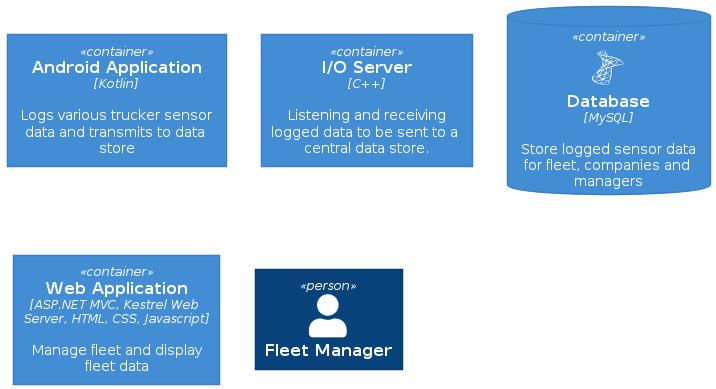
\includegraphics[width=6in]{../diag/container.png}
\caption{Container Diagram - Fleet tracking system}
\label{fig:container}
\end{figure}

\subsubsection{Data Model}
The entire system revolves around the effective abstraction and manipulation of logged fleet data.
MySQL is chosen as the \ac{rdbms} to realize a relational database model, as it is high performance and reliable.
Other \ac{rdbms}s (such as Microsoft SQL Server, PostgreSQL) offer comparable performance, but MySQL is chosen for familiarity.

The relational model is depicted in figure \ref{fig:erd}.
The model is designed to allow one company to have many managers and truckers. Each trucker can have many logs.

\subsubsection{Android Application}
Kotlin is the language of choice to write the android application due to its simplicity and mainstream Google support.

Truckers must receive an initial code from their managers' to register their devices.
Sensor readings are taken every two minutes, and stored into a lightweight database.
Finally, a connection is attempted with an \ac{io} server. If available, the database contents is emptied into via the \ac{io} server to the central system database.

\subsubsection{\Ac{io} Server}
C++ is chosen for the \ac{io} server, due to its high performance capabilities.
The \ac{io} server needs to listen and allow multiple asynchronous connections, during which log data is transmitted to the database.

\subsubsection{Web Application}
The \ac{mvc} architecture will be realized with the Microsoft ASP.NET framework.
This architecture allows for separation between business-logic, data models and viewing logic.
This is necessary to ensure that code related to displaying data is not mixed with code used for core logic, thereby separating and modularizing the functionality of different components in the system.

\pagebreak
\subsection{Subsystem components and Design}
Each container in figure \ref{fig:container} is subdivided into several core software components necessary to achieve the desired outcomes.
This is depicted through container diagrams, which makes up the third level of the C4 model.

\subsubsection{Android Application - lifecycle and software abstractions}
\begin{figure}[H]
\centering
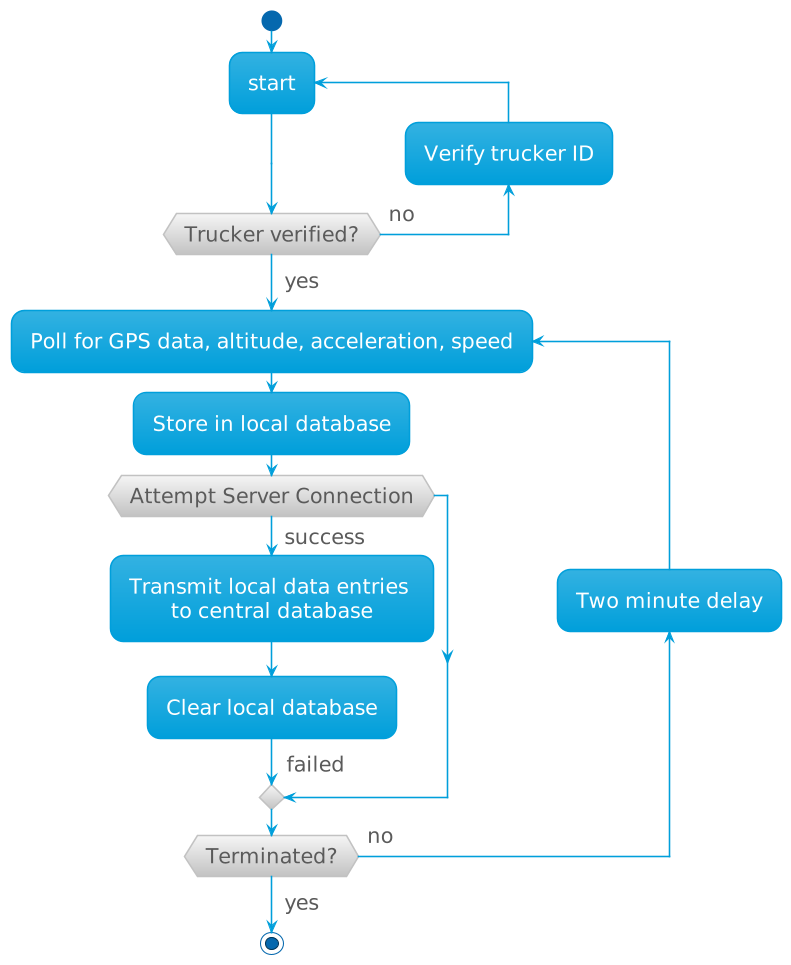
\includegraphics[scale=0.4]{../diag/android_activity.png}
\caption{Life-cycle - Android Application}
\label{fig:android_activity}
\end{figure}

The life cycle of the Android application is depicted in figure \ref{fig:android_activity}.
Initially, a check is performed to confirm that the trucker \ac{id} is in the central database, and is not duplicated.
If this \ac{id} is not valid, the trucker must request a valid \ac{id} from the fleet manager.

After this, the usual logging process is continued.
Data is polled from the available sensors and stored in a local database.
A connection is attempted with the \ac{io} server and the local database entries are transmitted to the server.
Upon successful transmission, the local database is cleared.
However, if a connection fails, the local database is not cleared.
This process loops continuously loops every two minutes.
 
\begin{figure}
\centering
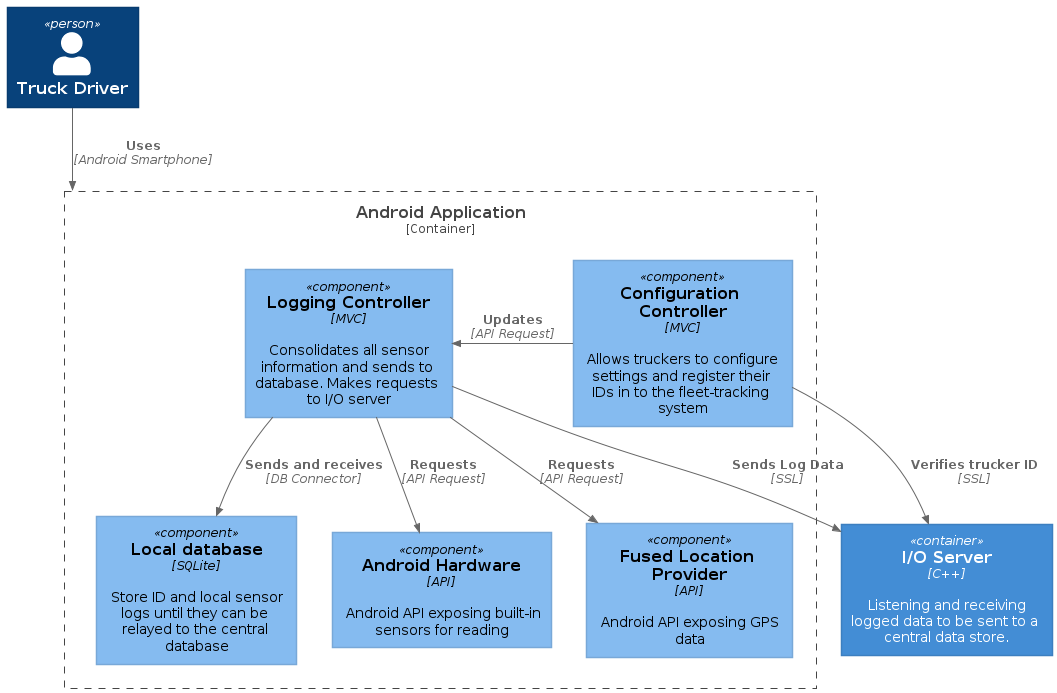
\includegraphics[width=6in]{../diag/android_component.png}
\caption{Component Diagram - Android Application}
\label{fig:android_component}
\end{figure}

The android application is designed with the \ac{mvvm} design pattern (detailed in figure \ref{fig:mvvm_layout}).
Figure \ref{fig:android_component} details software components (classes) that are clearly represented in the source code.
\begin{enumerate}
\item \textbf{Main Activity}\\
The main activity renders the application's main user interface to the user.
This component mainly implements \Ac{ui}-handling logic, with callbacks which are primarily event-driven (when users press buttons for example).
\item \textbf{Main View Model}\\
Activities have short lifetimes and are often recreated when users switch between applications or tilt their screens.
Due to this, a manager class is necessary to ensure data is persisted - this is achieved by the view model.
\item \textbf{Tracking Service}\\
The tracking service is toggleable service which runs in the background as a foreground service.
It polls acceleration and location data via interfaces made available in the Android \ac{api}.
It runs without requiring the main activity to be open on the user's screen.
\item \textbf{Main Repository}\\
Multiple components require performing \ac{io} operations.
To avoid repetition and prevent conflicts, the main repository performs these operations.
It exists as a singleton and is injected into calling objects with \ac{di}.
\item \textbf{Room - Object Relational Mapper}\\
Android's room abstraction layer provides a data class abstraction of data stored in the SQLite database.
This abstraction makes it easier to work with data in language-specific data structures.
Room provides a \ac{dao} to the main repository for database operations.
\item \textbf{SQLite database}\\
SQLite is a lightweight go-to database provider for Android applications.
It is ideal for storing medium to small sized volumes of data.
\item \textbf{Server Connector}\\
The server connector provides \ac{ssl} socket communication with the central \ac{io} server.
Request objects are serialized into text data streams for transmission.
Likewise, server responses are deserialized into response objects and handled appropriately.
\item \textbf{Shared Preferences}\\
Android's \textit{SharedPreferences} library provides an \ac{api} for the purposes of reading/writing key value data in a file on disk.
This is used for storing user configuration, such as identity and upload preferences, which aren't appropriate for a database.
\end{enumerate}

These components are necessary for realizing a modular, extendable application.

\pagebreak
\subsubsection{\Ac{io} Server}
The typical life cycle view of the \ac{io} server is depicted in figure \ref{fig:IO_activity}.
A secure connection must be made due to the sensitive nature of \ac{gps} data.
\begin{itemize}
\item A session is assigned for the lifetime of the communication, which handles the three-way \ac{ssl} handshake, ensuring the client trusts the server. The incoming payload is decrypted.
\item A request handler parses (and deserializes) the decrypted payload, which queries the database to generate an appropriate serialized response.
\item The response is sent back to the client and the session is terminated.
\end{itemize}

The popular C++ library, \textit{asio} can implement the above workflow in an asynchronous manner.

\begin{figure}
\centering
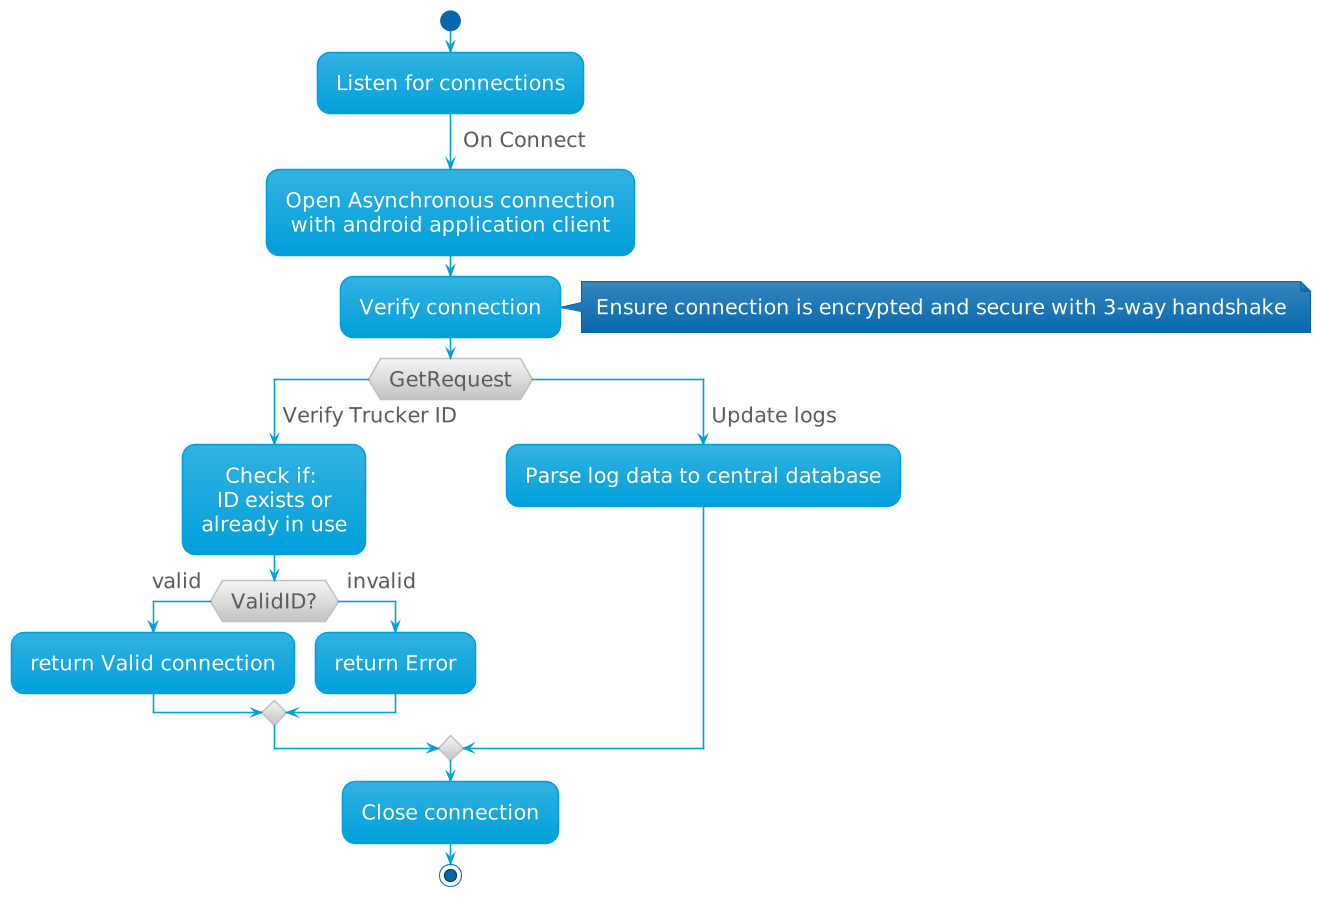
\includegraphics[width=6in]{../diag/IO_activity.png}
\caption{Life cycle - \Ac{io} Server}
\label{fig:IO_activity}
\end{figure}

\begin{figure}[H]
\centering
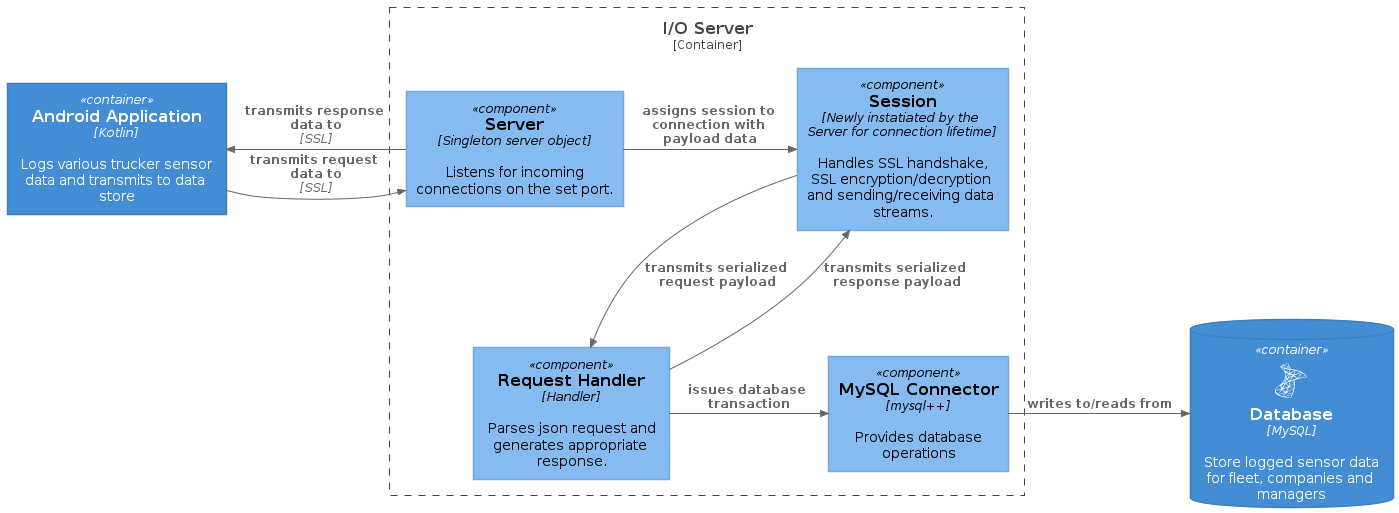
\includegraphics[width=6in]{../diag/IO_component.png}
\caption{Component Diagram - \Ac{io} Server}
\label{fig:IO_component}
\end{figure}

Figure \ref{fig:IO_component} depicts the software abstractions and program structure used to realize the \ac{io} server.
The codebase clearly contains these low-level abstractions.
\begin{enumerate}
\item \textbf{Server}\\
The server object listens for incoming \ac{tcp} connections.
Upon receiving a connection, a new session is instantiated to handle to communication.
\item \textbf{Session}\\
The session performs the necessary encryption, decryption and three-way handshake required for the \ac{ssl} protocol.
The session reads in and writes out the serialized payload on the socket.
\item \textbf{Request Handler}\\
The request handler performs serialization and deserialization.
It processes the request and queries the database appropriately.
\item \textbf{MySQL Connector}\\
An interfacing object to the MySQL database.
\end{enumerate}

\pagebreak
\subsubsection{\ac{json} protocol}
Figure \ref{fig:json_protocol} depicts the structure of the protocol used for communication between the \ac{io} server and the android client.
The communication follows a \ac{rest}ful structure, which is common for web communications.
That is, communication requires no knowledge of intermediate state.
One request is enough to complete the required transactions, after which an appropriate response is sent back to the client.

\begin{figure}[H]
\centering
    \subfigure[Request payload]
    {
        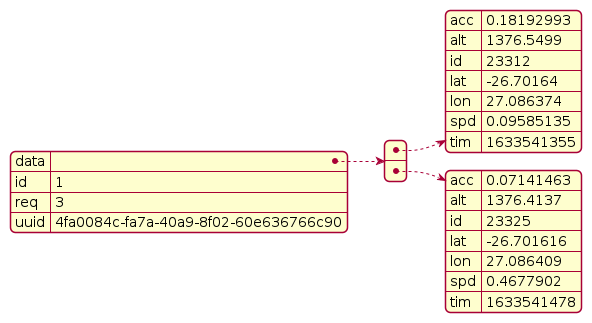
\includegraphics[scale=0.5]{../diag/json_request.png}
        \label{fig:json_request}
    }
    \subfigure[Response payload]
    {
        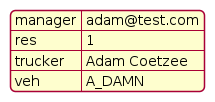
\includegraphics[scale=0.5]{../diag/json_response.png}
        \label{fig:json_response}
    }
\caption{\Ac{json} protocol}
\label{fig:json_protocol}
\end{figure}


\begin{itemize}
\item The client makes a request in \ac{json} form, as shown in figure \ref{fig:json_request}.
It contains \ac{id} information about the client, a request code and any payload data (typically tracking data). Possible requests include verifying \ac{id}, sending log updates and registering new \ac{id}s.
\item The server appropriately handles the request (based on request code) and generates an appropriate response. Usually the response will just contain the response code, but it may sometimes carry extra information (as seen in figure \ref{fig:json_response}).
Responses can return a fail, ok, invalid credential, database connection error or parsing error status.
\end{itemize}

 This communication is realized through \ac{ssl} sockets over the network.

\pagebreak
\subsubsection{Web Application}
The web application is modeled with the \ac{mvc} design pattern, which allows for following \ac{soc} principles.
Backend logic is realized in C\# using Microsoft's \textit{ASP.NET} framework.
Web pages are generated with a combination of C\#, JavaScript and \ac{html} styled with \ac{css}.

\begin{figure}[H]
\centering
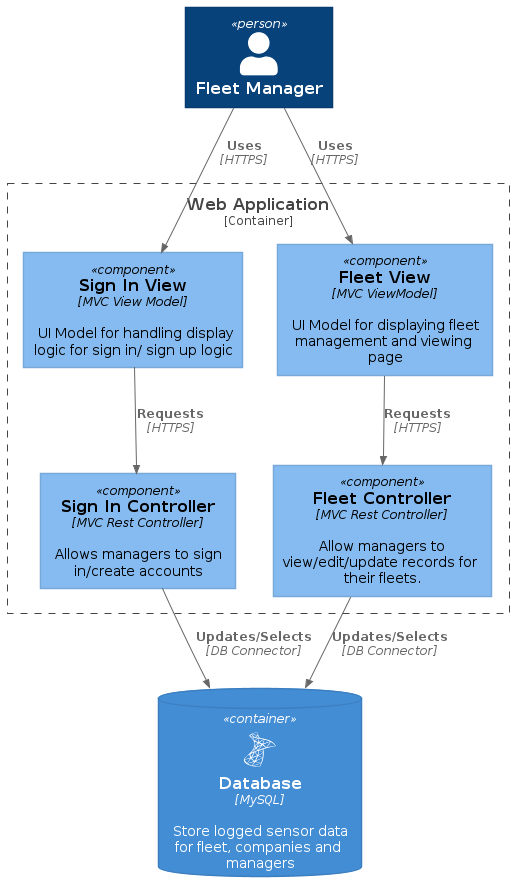
\includegraphics[width=6in]{../diag/webapp_component.png}
\caption{Component Diagram - Web Application}
\label{fig:webapp_component}
\end{figure}

Figure \ref{fig:webapp_component} depicts the architectural arrangement of the web application.
\begin{enumerate}
\item \textbf{ASP.NET Identity Views and Controller}\\
Microsoft provides a professional library for handling user access, known as \textit{ASP.NET Identity}.
This library handles logic for user registration, signing in and account editing.
In addition, there is support for email verification and two-factor authentication.
Identity also implements logic for restricting access to pages, ensuring managers can only view data related to their fleets'.

\item \textbf{DB Context and MySQL database}\\
Microsoft's \textit{Entity Framework} provides the abstraction of data as 'entites' to be represented by models (data classes in code).
This makes for easier interaction with data in code.
The back-end database in use is MySQL.

\item \textbf{Fleet Models}\\
The Fleet Models are a set of data classes used for the abstraction of data entities in code.
They allow for the easy passing of data from controllers to views.
An extra view model class is used for viewing truckers.
Since viewing truckers requires extra processing of trucker information logs, an extra class is utilized to handle this processing.

\item \textbf{Fleet Controller}\\
User interactions from any of the fleet views results in \ac{http} requests issued to the Fleet Controller.
The Controller has multiple methods for handling different \ac{http} requests.
Upon receiving a routed request, it selects the appropriate method and queries the appropriate fleet data from the database abstraction layer.
The results of the query are populated into one of the models, and the model is returned to the view.

\item \textbf{Fleet Views}\\
Multiple views are returned by the Fleet Controller depending on request, and act as the \ac{ui} component visible to the user.
Each view only handles the necessary logic required for displaying data returned as a model from the controller.
The \ac{ui} is rendered as \ac{html}, with backend C\# logic utilized to dynamically render view components, such as tables.
Additional \ac{ui} logic is realized with JavaScript.

\begin{enumerate}
\item \textbf{Index}\\
The Index view displays a list of all truckers registered by the manager.
It provides an interface for resetting each trucker's Android \ac{id}.

\item \textbf{Add Trucker}\\
The "Add Trucker" page provides an \ac{html} form for the purposes of adding trucker's to the fleet.
Details about the trucker such as name and vehicle number can be added.

\item \textbf{Set Rules}\\
The "Set Rules" page allows the manager to define custom rules defining unacceptable driving behavior, including maximum speed and acceleration.

\item \textbf{View Trucker}\\
The "View Trucker" page displays details about the trucker's activities for an adjustable time period.
A table is used to group location data into individual trips.
This table is generated by means of a grouping algorithm to segment the driver's activities into separate trips, and includes information such as waiting time, average speed and indications of any rule breaks.

In addition, each trip is drawn in a map using the \textit{Google Maps JavaScript \ac{api}}.
This provides a neat visual representation of Trucker activities.

\item \textbf{View Trip}\\
The "View Trip" page allows for detailed statistical analysis of individual trips.
It provides percentile analysis and graphs showcasing the trucker's speed, acceleration and altitude.
\end{enumerate}

\end{enumerate}

\pagebreak
\subsubsection{MySQL Database and Entity relationships}
The central backend \ac{rdbms} used is MySQL.
A relational data structure is utilized, as shown in figure \ref{fig:erd}.
Relational modeling allows for logical structuring and integrity of the data.

\begin{figure}[H]
\centering
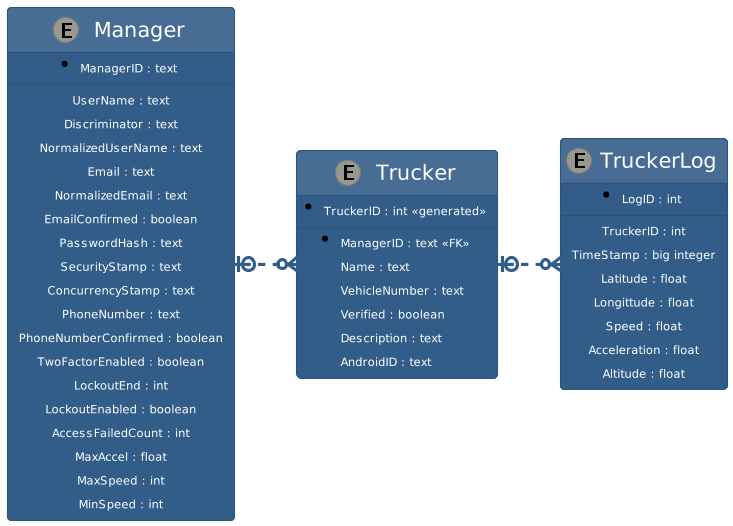
\includegraphics[scale=0.5]{../diag/erd.png}
\caption{Fleet Tracking System - Entity Relationship Diagram}
\label{fig:erd}
\end{figure}

The Manager entity represents the web application user, and contains various fields used for storing the manager's identity.
In addition, the fields "MaxAccel", "MaxSpeed" and "MinSpeed" define rules for good trucker behavior.

One manager can manage multiple truckers (or none), therefore enforcing a zero-to-many relationship.
Similarly, each trucker can have multiple (or no) logs.
The Trucker entity stores information about each trucker.
The TruckerLog entity stores the entries of each log in the database.

Unix timestamps are used for identifying the time of each log, which is convenient and saves on storage, as only 8 bytes are required.
Additionally, single precision float precision provides location precision within 2.37 meters\cite{noauthor_required_nodate} in the worst case, making it adequate it for this application, while saving on storage. Double precision is more computationally expensive for little benefit.

\subsection{Data Processing}
The main focus and purpose of the system is to generate useful information for managers which can be used to optimize their fleets.
The raw tracking data alone doesn't give the clearest indication of trucking behavior.

\subsubsection{Aggregating nearby logs}
Determining when trucker's have stopped is useful for segmenting trips.
Grouping trips into different segments gives a clear idea of what truckers are doing.
To this end, an algorithm is designed with this goal in mind.

It is first helpful to remove logs where an insignificant distance is traveled, or where the user is stationary.
Algorithm \ref{algo_agg} achieves this, by creating a new list where the distance between each log is some \textit{MINDISTANCE} away from the previous log. A threshold of 150 meters is chosen.

\SetKwComment{Comment}{/* }{ */}

\begin{algorithm}
\SetKwData{Left}{left}\SetKwData{This}{this}\SetKwData{Up}{up}
\SetKwFunction{Union}{Union}\SetKwFunction{FindCompress}{FindCompress}
\SetKwInOut{Input}{input}\SetKwInOut{Output}{output}
\Input{List of chronologically Sorted Logs}
\Output{Aggregated list of logs, where each log is a significant distance away from the next}

\BlankLine
\emph{Generate list of aggregated logs far enough away from each other}\;
$AggregatedLogs.Append \gets LogsSortedByDate[0]$\;
$LastLog \gets LogsSortedByDate[0]$\;
\For{$i\leftarrow 0$ \KwTo $LogsSortedByDate.Length$}{
    \If{$Distance(LogsSortedByDate[i], LastLog)\geq MINDISTANCE$}
    {
        $AggregatedLogs.Append \gets LogsSortedByDate[i]$\;
        $LastLog \gets LogsSortedByDate[i]$\;
    }
}
\caption{Aggregating logs close to each other}\label{algo_agg}
\end{algorithm}\DecMargin{1em} 

\subsubsection{Defining trips between stop locations}
The aggregated list of logs determined in algorithm \ref{algo_agg} is then used to group together trips.
A trip is defined as the logs between consecutive stops.
A stop is defined using the time difference between two distance-aggregated logs, where the time between each log is greater than some threshold (\textit{MINTIME}).
A value of 5 minutes is chosen to designate a stop.
Algorithm \ref{algo_trips} shows the algorithm used to determine this.

\begin{algorithm}[H]
\SetKwData{Left}{left}\SetKwData{This}{this}\SetKwData{Up}{up}
\SetKwFunction{Union}{Union}\SetKwFunction{FindCompress}{FindCompress}
\SetKwInOut{Input}{input}\SetKwInOut{Output}{output}
\Input{List of chronologically, aggregated Logs, where consecutive logs are a minimum distance away from each other}
\Output{List of trips(segments) defined from some start log to some end log}

\BlankLine
\emph{Use aggregated list to determine individual \textit{trips} separated by stopping points}\;
$startLogCount \gets 0$ \Comment*[r]{The start of a trip}
\For{$i\leftarrow 0$ \KwTo $AggregatedLogs.Length-1$}{
    \If{$TimeDifference(AggregatedLogs[i+1], AggregatedLogs[i])\geq MINTIME$}
    {
        \eIf{$i == 0$}
        {
            \emph{If the first log is a stop, don't start the trip from here}
            $startLogCount \gets startLogCount+1$\;
        }
        {
            \emph{Add a trip, starting from the previous start log till the current log}\;
            $Segments.Append \gets AggregatedLogs[startLogCount],AggregatedLogs[i]$\;
            \emph{the next trip will start from the next aggregated log}\;
            $startLogCount \gets i+1$\;
        }
    }
}
\caption{Grouping logs into trips}\label{algo_trips}
\end{algorithm}\DecMargin{1em} 

The \textit{Segments} determined in algorithm \ref{algo_trips} can be tabulated to give details of each trip the trucker performed.

\pagebreak
\subsection{\Acf{ui} Design}
The primary goal of \ac{ui} design is to make the interface clear and intuitive for users.

\subsubsection{Android Application}
Figure \ref{fig:android_ui} depicts the blueprint of Android application's \ac{ui}.
\Ac{xml} is used in Android to define the positioning of elements in the layout.
\begin{figure}[H]
\centering
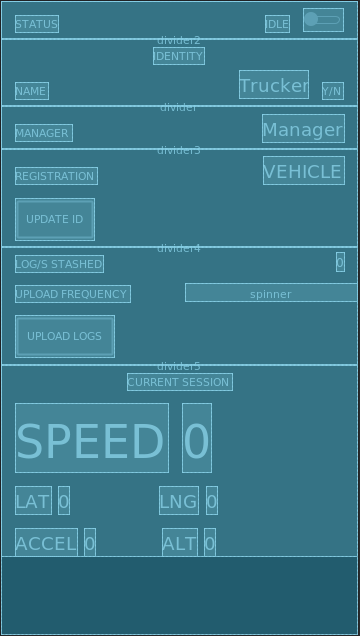
\includegraphics[scale=0.65]{android_ui.png}
\caption{Android Application - \ac{ui}}
\label{fig:android_ui}
\end{figure}

To account for different screen sizes, a Constraint layout is used, in which elements are tied to edges or specific points in the layout's geometry.
Elements are places relative to each other, and will dynamically adjust when tilting the screen.
The constraint layout is placed within a scroll view to allow scrolling if the elements can not fit on the screen.

The \ac{ui} allows the user to toggle the tracking service.
It provides information about the trucker and his/her manager.
An interface is provided for toggling upload frequency of logs.
Finally, the current sensor readings are displayed.

\subsubsection{Web Application}
\begin{figure}
\centering
    \subfigure[Fleet index page]
    {
        \centering
        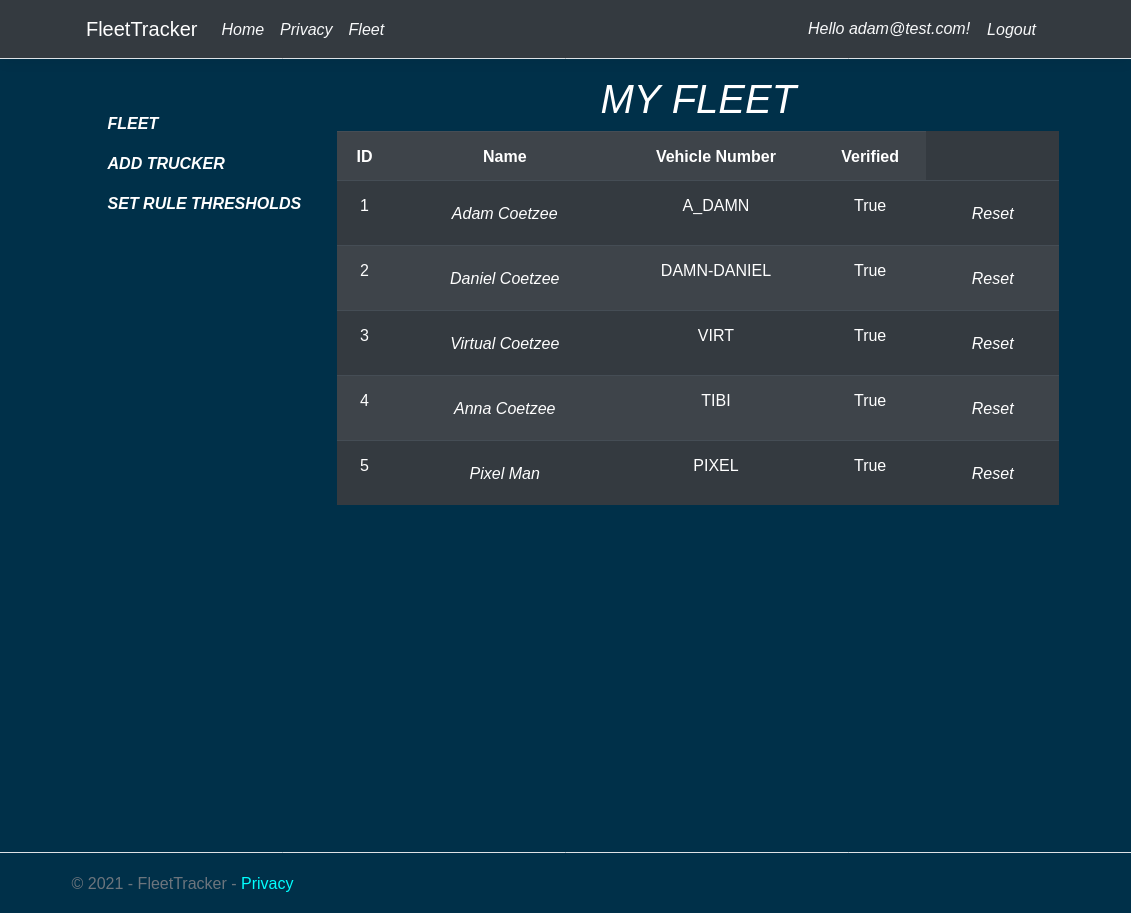
\includegraphics[width=2.5in]{fleet_index.png}
        \label{fig:fleet_index}
    }
    \subfigure[Add Trucker]
    {
        \centering
        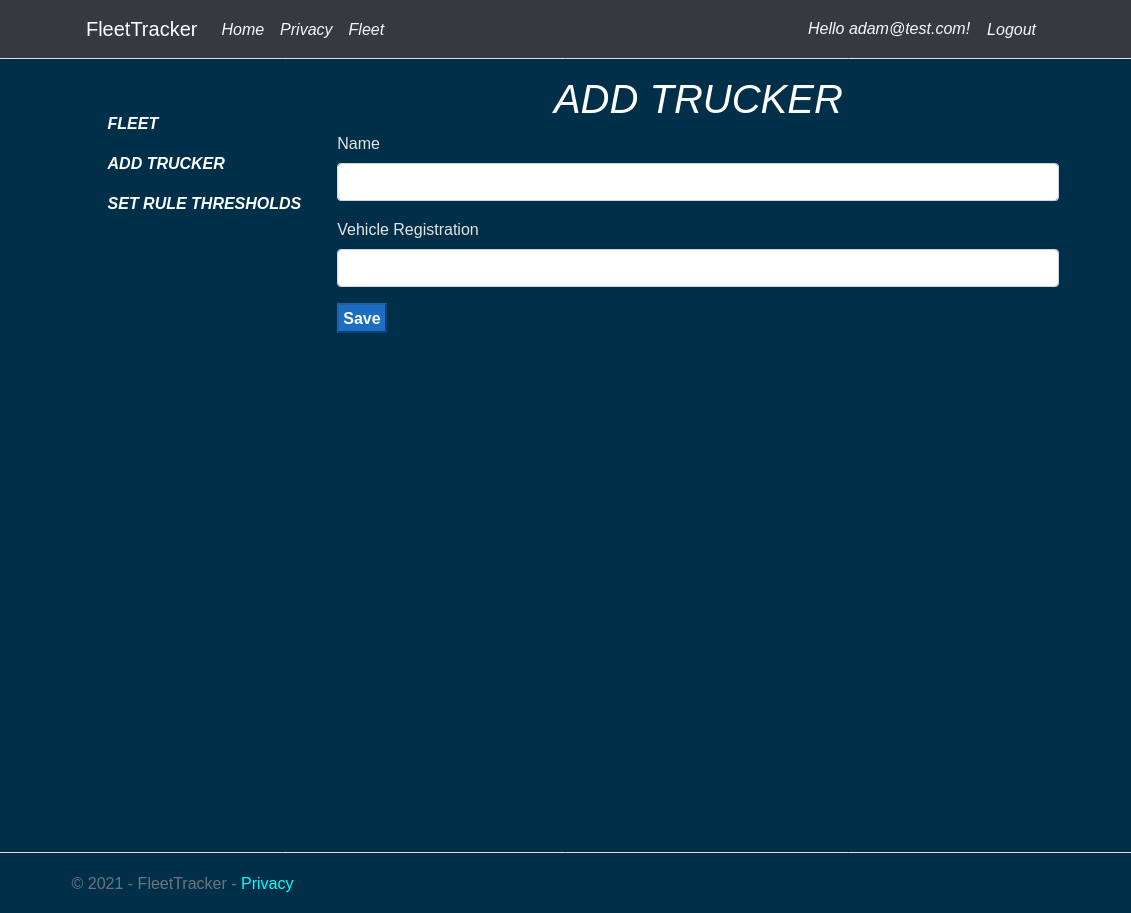
\includegraphics[width=2.5in]{fleet_add_trucker.png}
        \label{fig:fleet_add_trucker}
    }\\
    \subfigure[Set rules]
    {
        \centering
        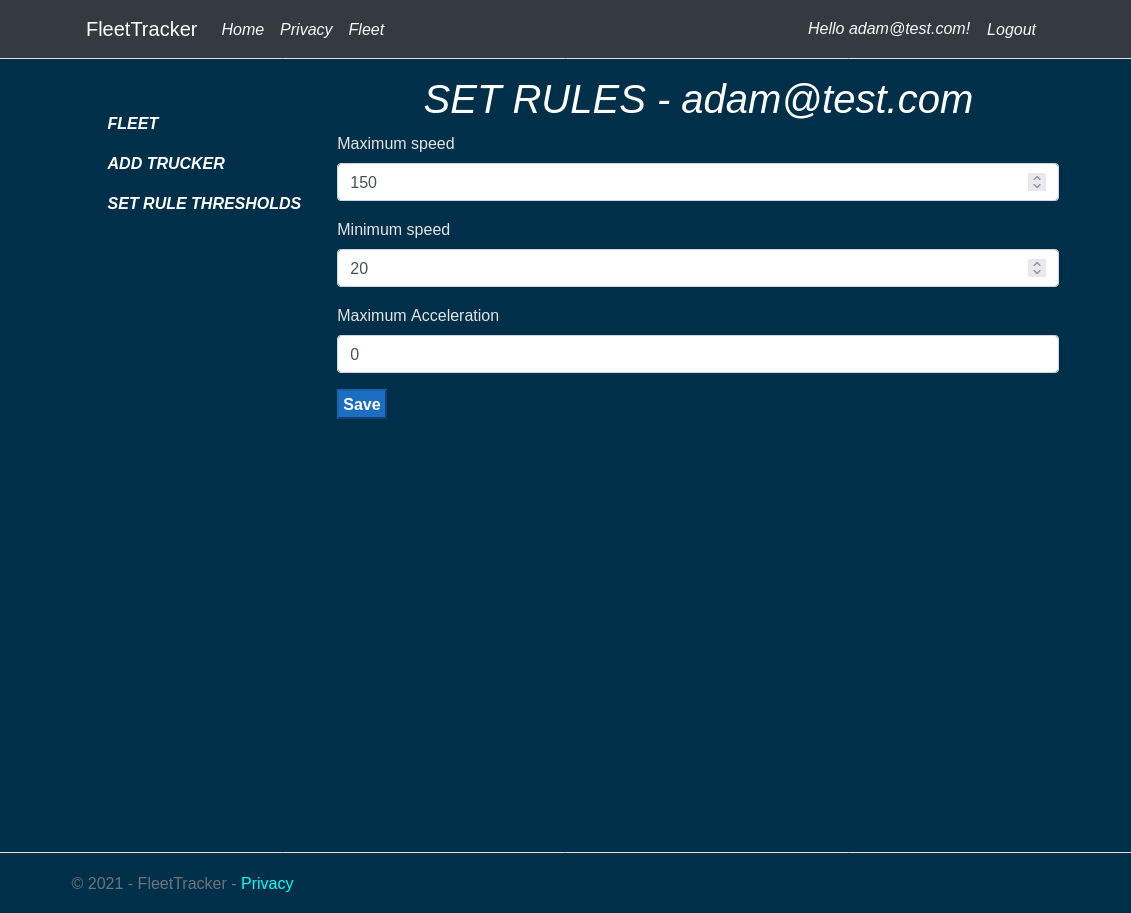
\includegraphics[width=2.5in]{fleet_set_rules.png}
        \label{fig:fleet_set_rules}
    }
    \subfigure[View Trucker]
    {
        \centering
        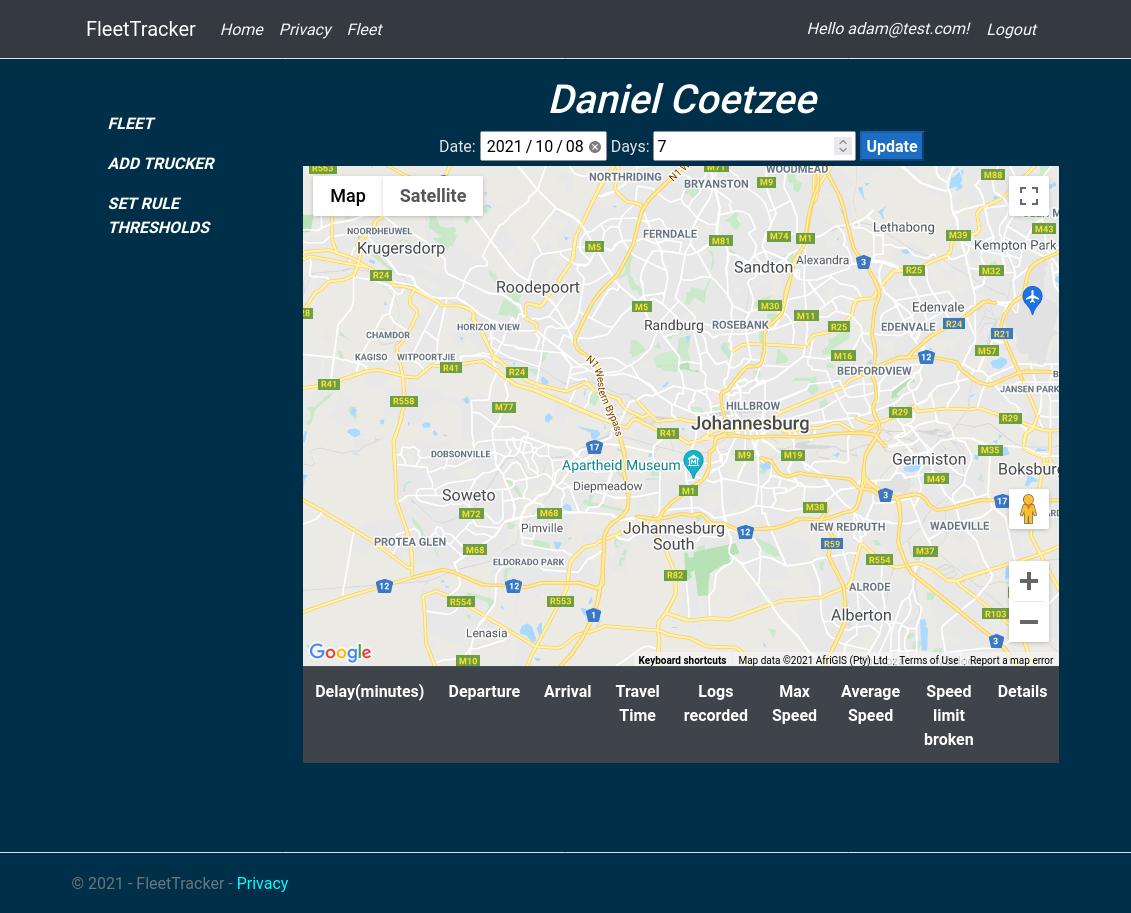
\includegraphics[width=2.5in]{fleet_view_trucker.png}
        \label{fig:fleet_view_trucker}
    }\\
    \subfigure[View Trip]
    {
        \centering
        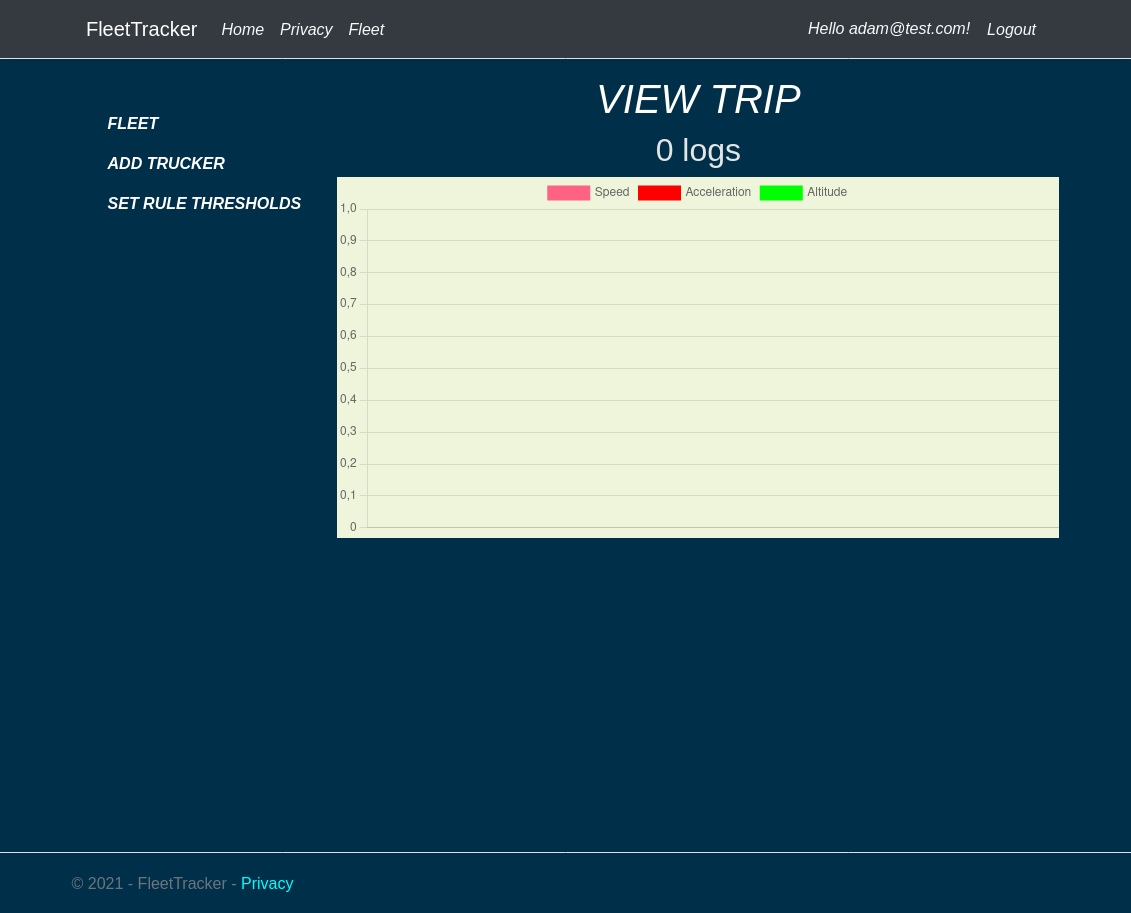
\includegraphics[width=2.5in]{fleet_view_trip.png}
        \label{fig:fleet_view_trip}
    }
\caption{Web application - Pages}
\label{fig:web_app_pages}
\end{figure}

Figure \ref{fig:web_app_pages} depicts the main pages used by managers for manipulating and viewing their fleets.
The web pages are designed using \ac{html} elements, which are style in \ac{css} aided by the \textit{Bootstrap} library which provides elegant \ac{css} presets.

\Ac{html} elements are spaced using \textit{div} containers in a grid layout.

\begin{itemize}
\item The index page, seen in figure \ref{fig:fleet_index} displays a list of truckers in the managers fleet. Managers can reset trucker \ac{id}s and navigate to individual trucker pages.
\item The "Add Trucker" page, in figure \ref{fig:fleet_add_trucker} allows managers to add new trucker entries.
\item The "Set Rules" page in figure \ref{fig:fleet_set_rules} allows managers to set rule thresholds for defining good behavior.
\item The "View Trucker" page, in figure \ref{fig:fleet_view_trucker} displays a map and table for displaying information about trips.
\item The "View Trip" page, in figure \ref{fig:fleet_view_trip} contains a graph for viewing statistics for trips.
\end{itemize}

\pagebreak

\section{Implementation}
This section considers the implementation and realization of the design.
Upon completion, the system is deployed to a \Ac{vps}, allowing for the service to be accessed on the internet.

\subsection{Android Application}
Figure \ref{fig:android_app_implementation} depicts the functionality and layout of the implemented android application.
Screenshots are taken of the application running in an Android emulator.

\begin{figure}[H]
\centering
    \subfigure[Idle state]
    {
        \centering
        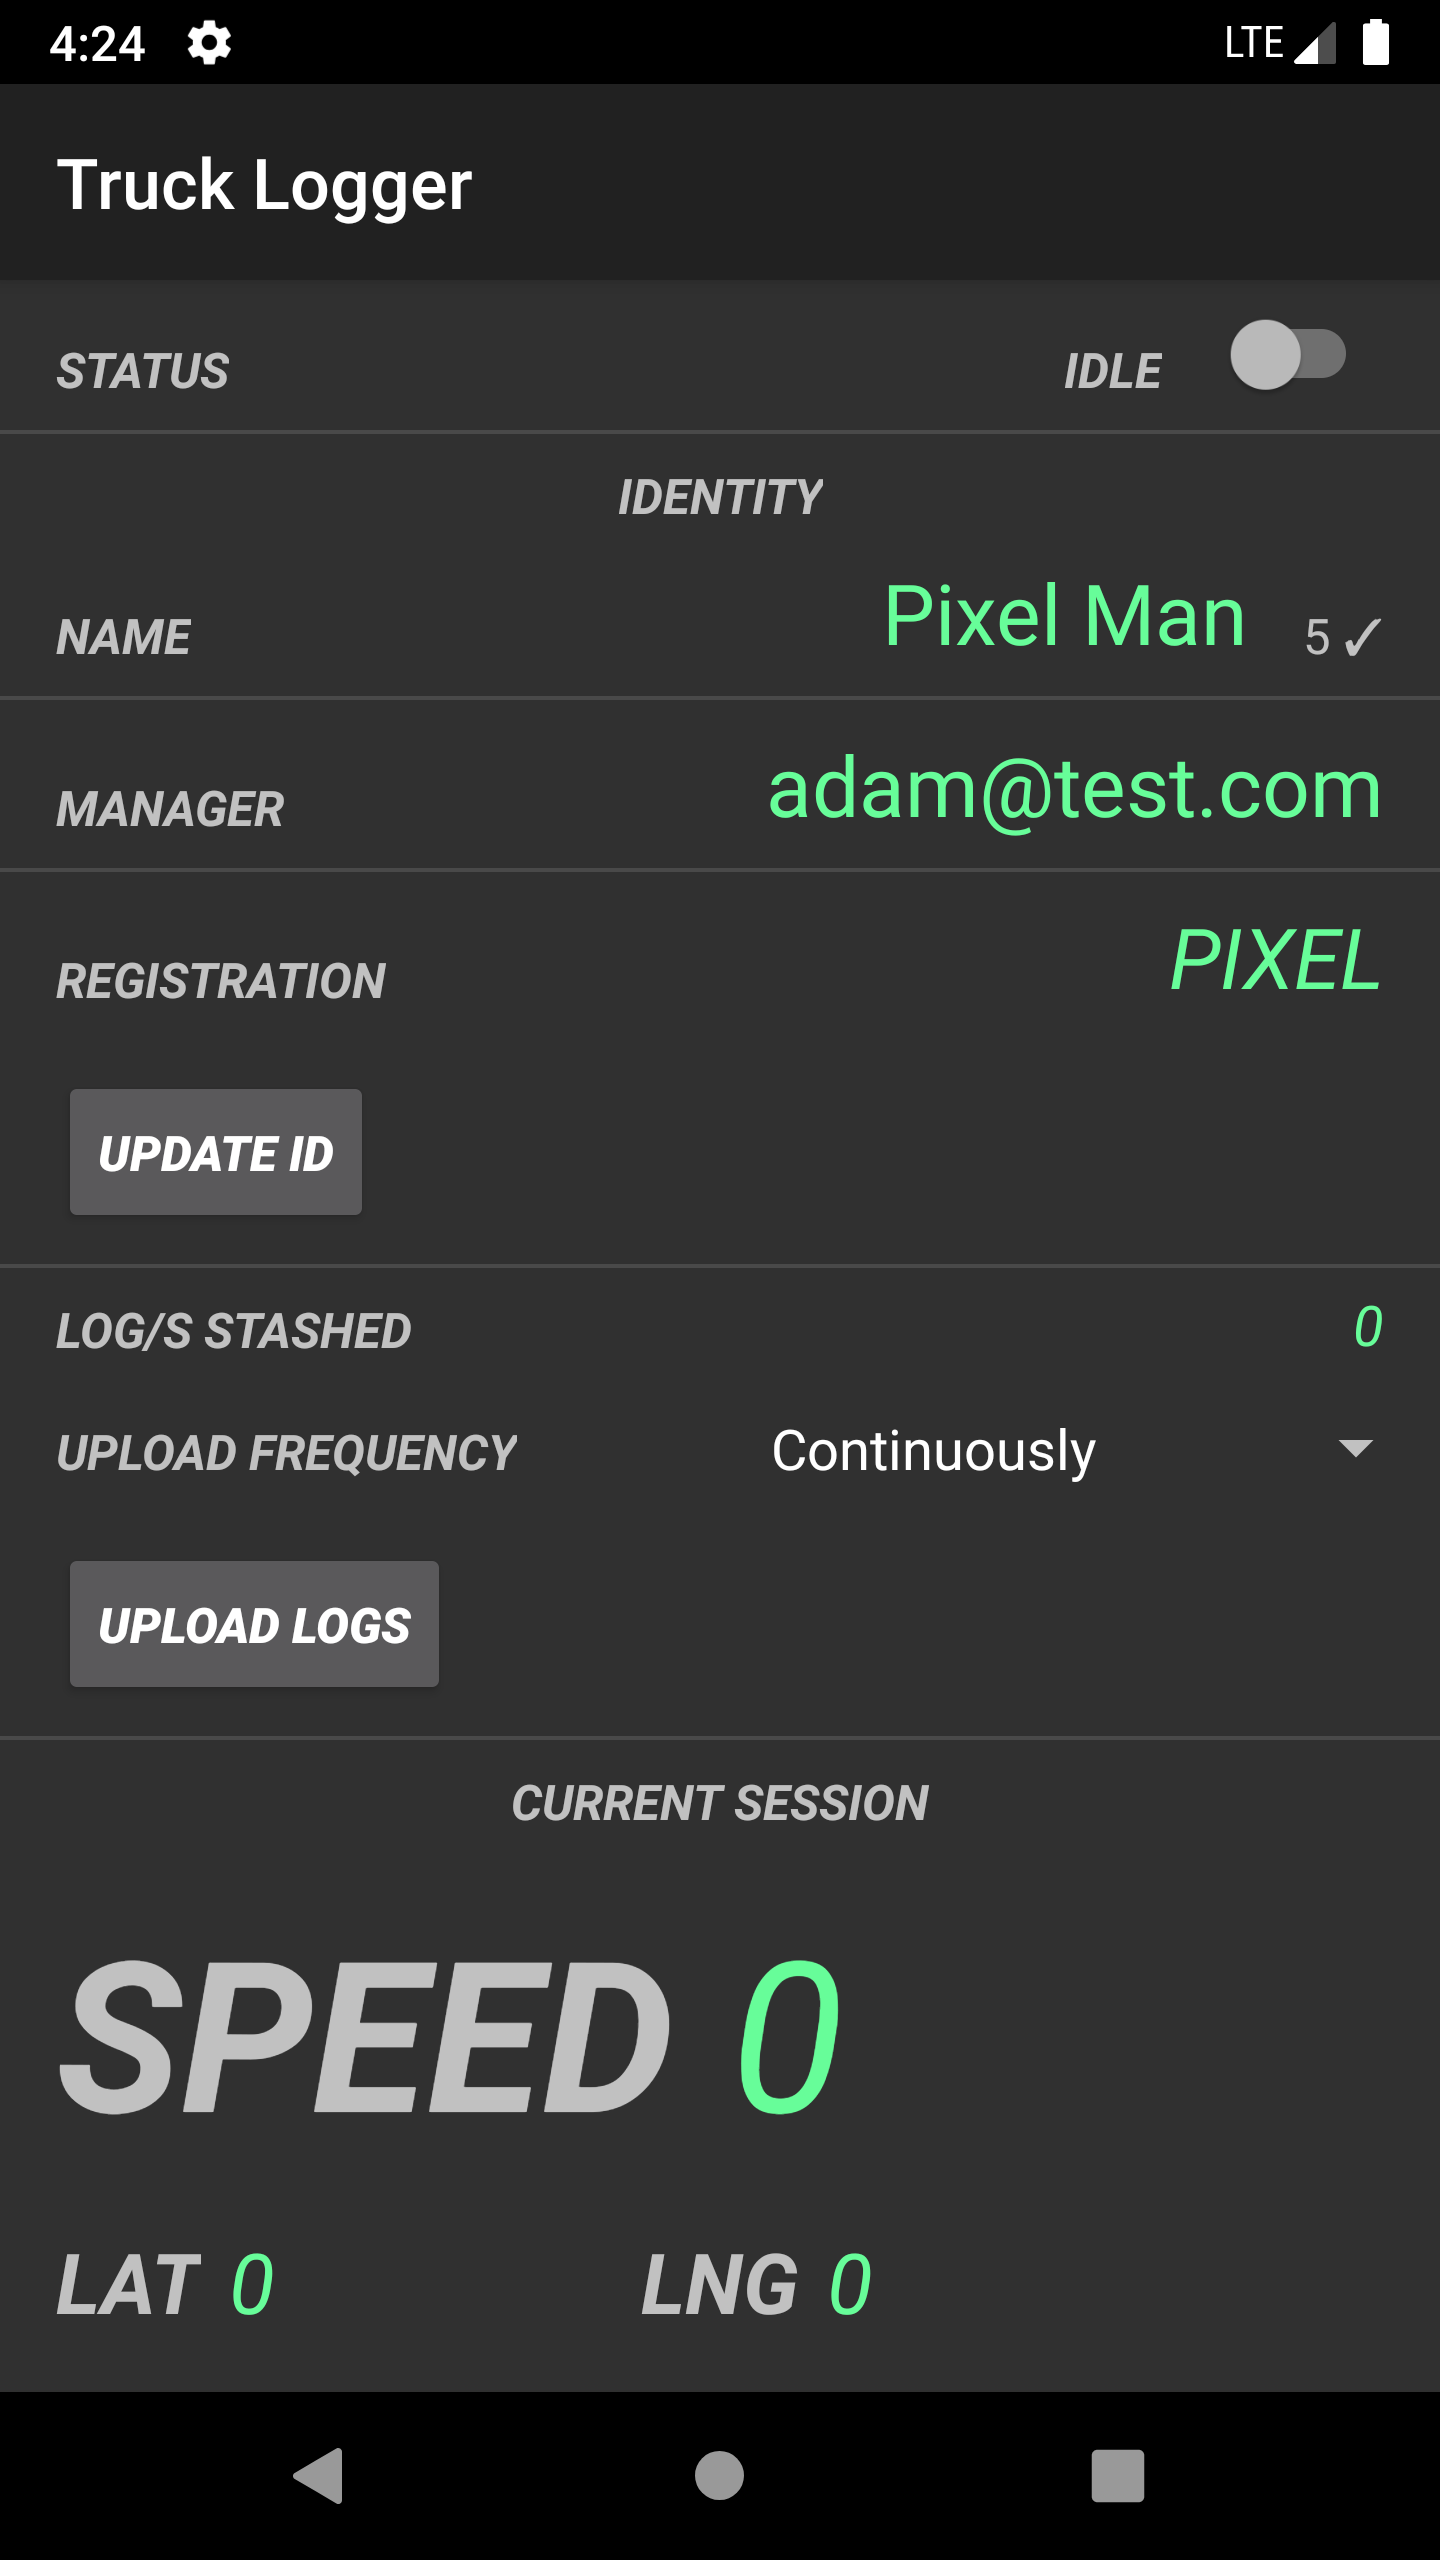
\includegraphics[height=2.5in]{android_app_idle.png}
        \label{fig:android_app_idle}
    }
    \subfigure[Running state]
    {
        \centering
        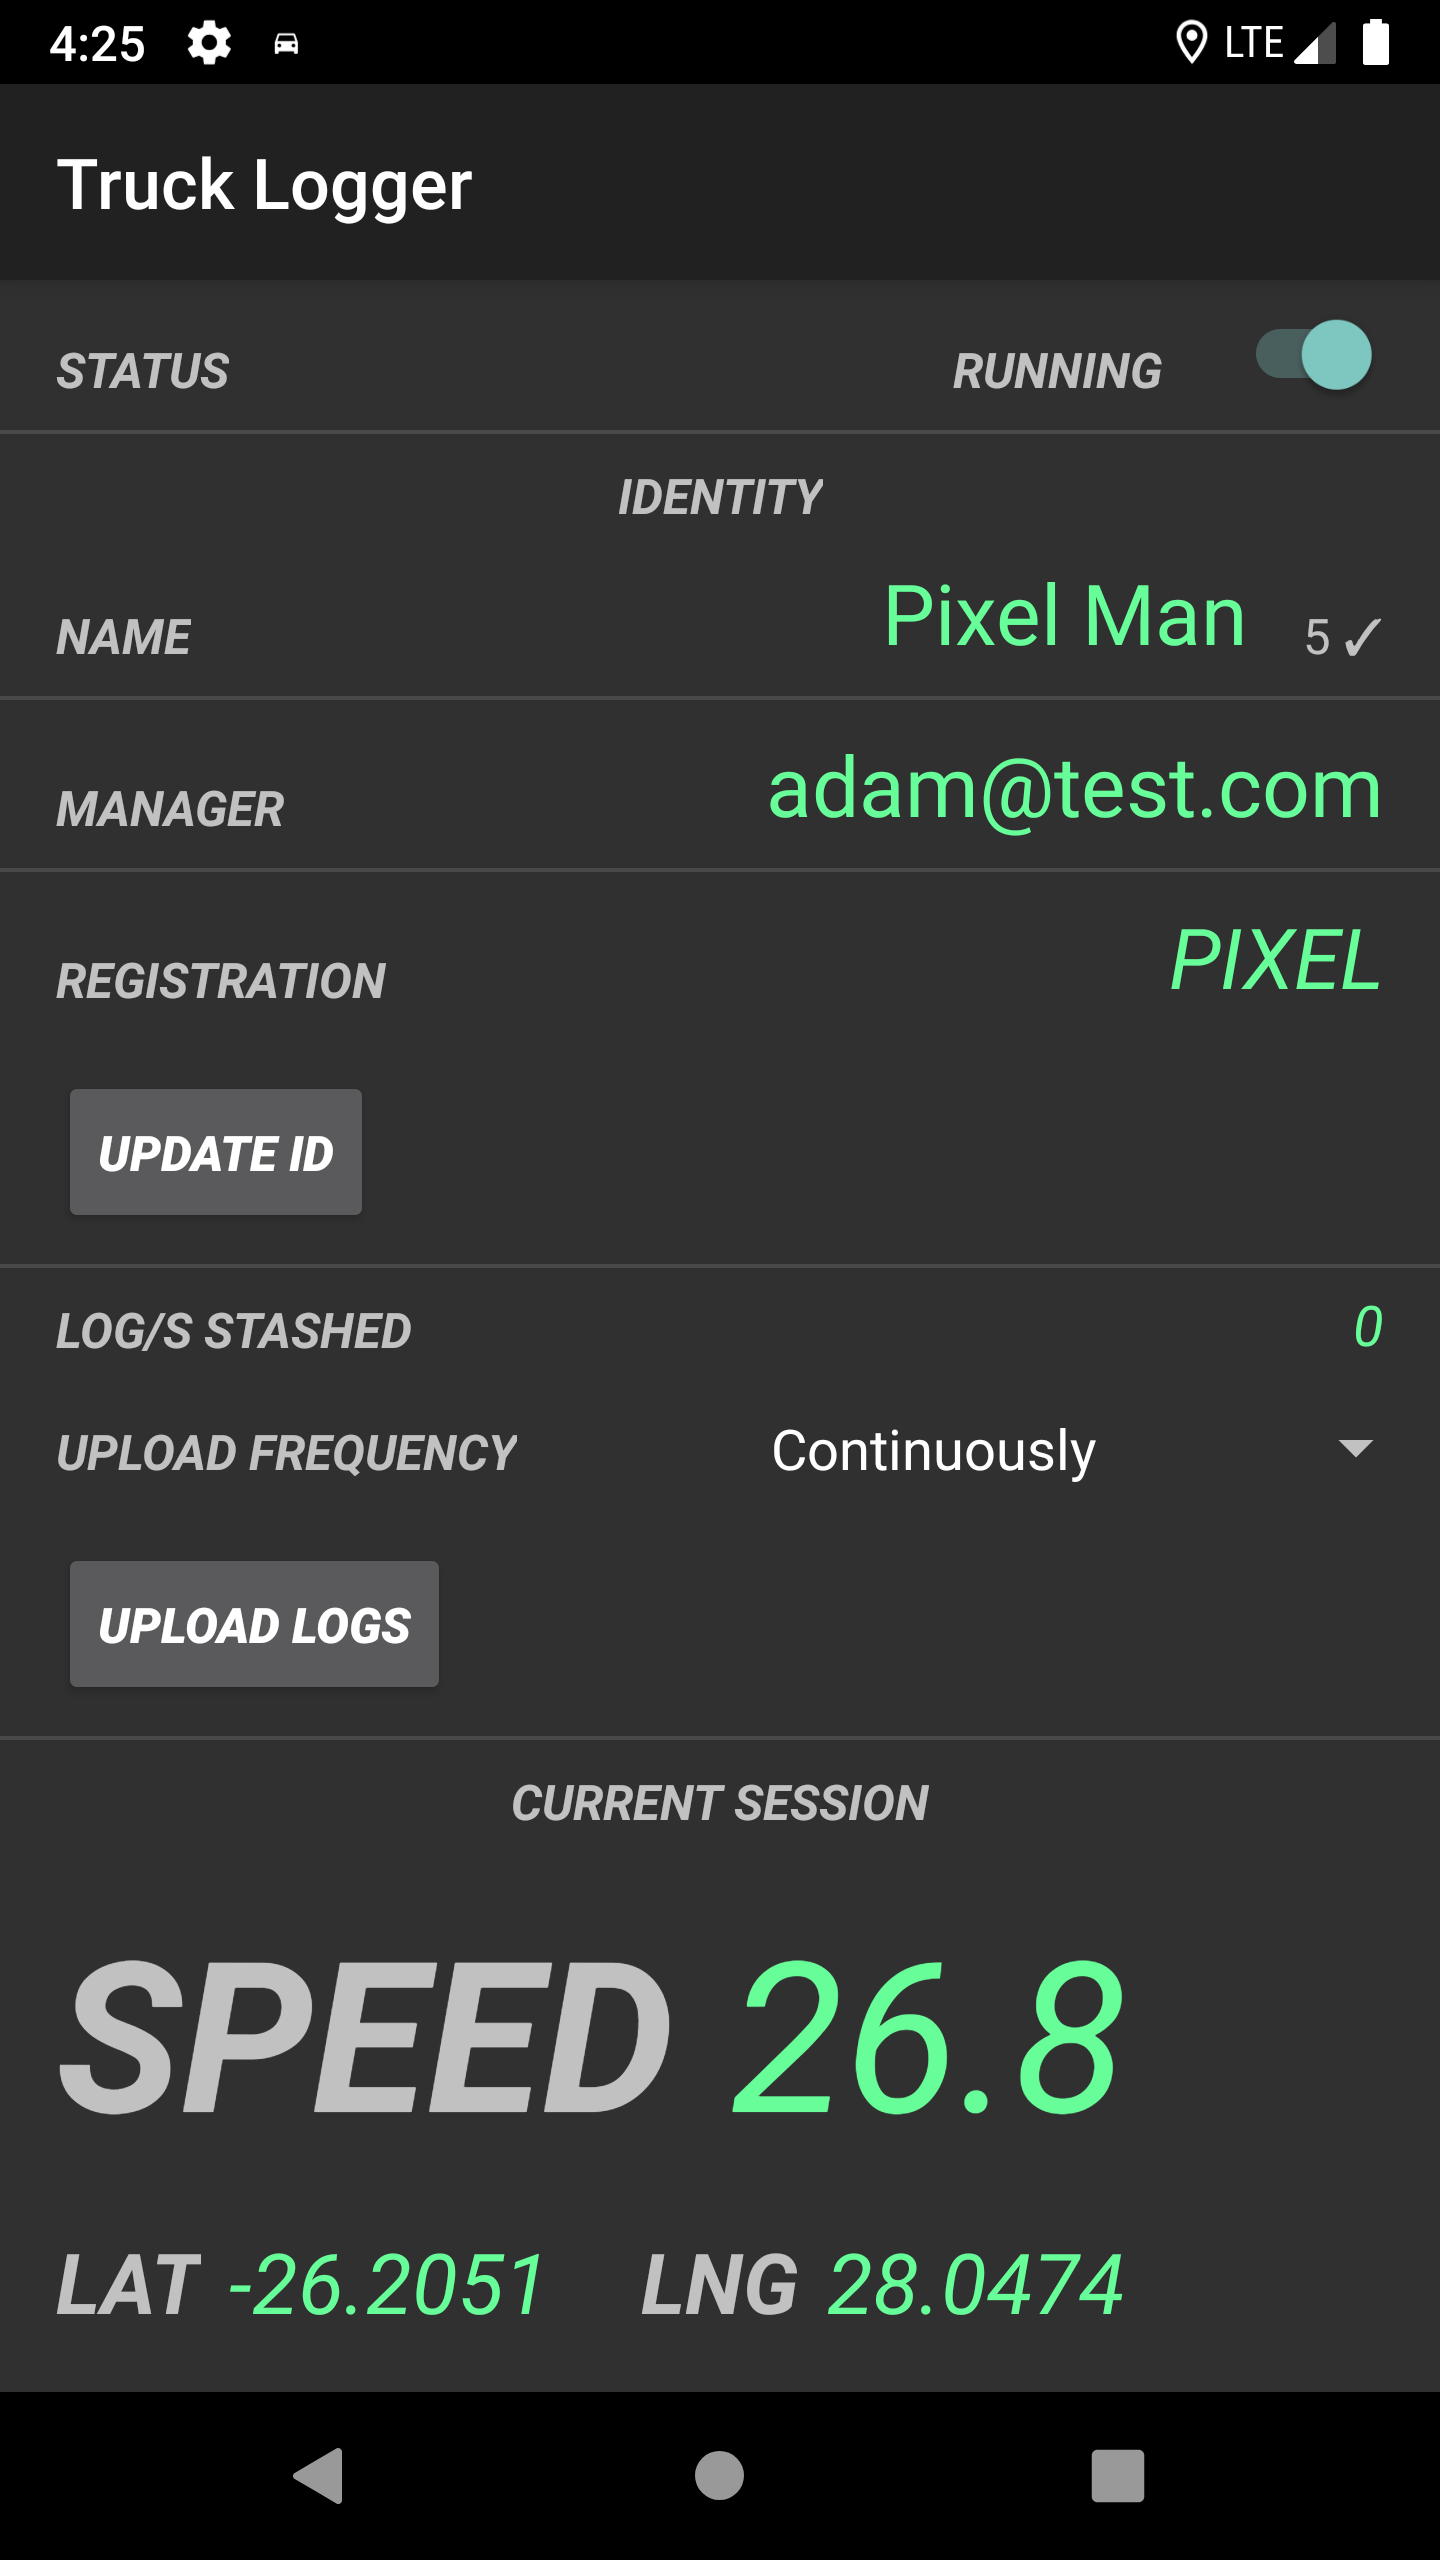
\includegraphics[height=2.5in]{android_app_running.png}
        \label{fig:android_app_running}
    }\\
    \subfigure[Background operation]
    {
        \centering
        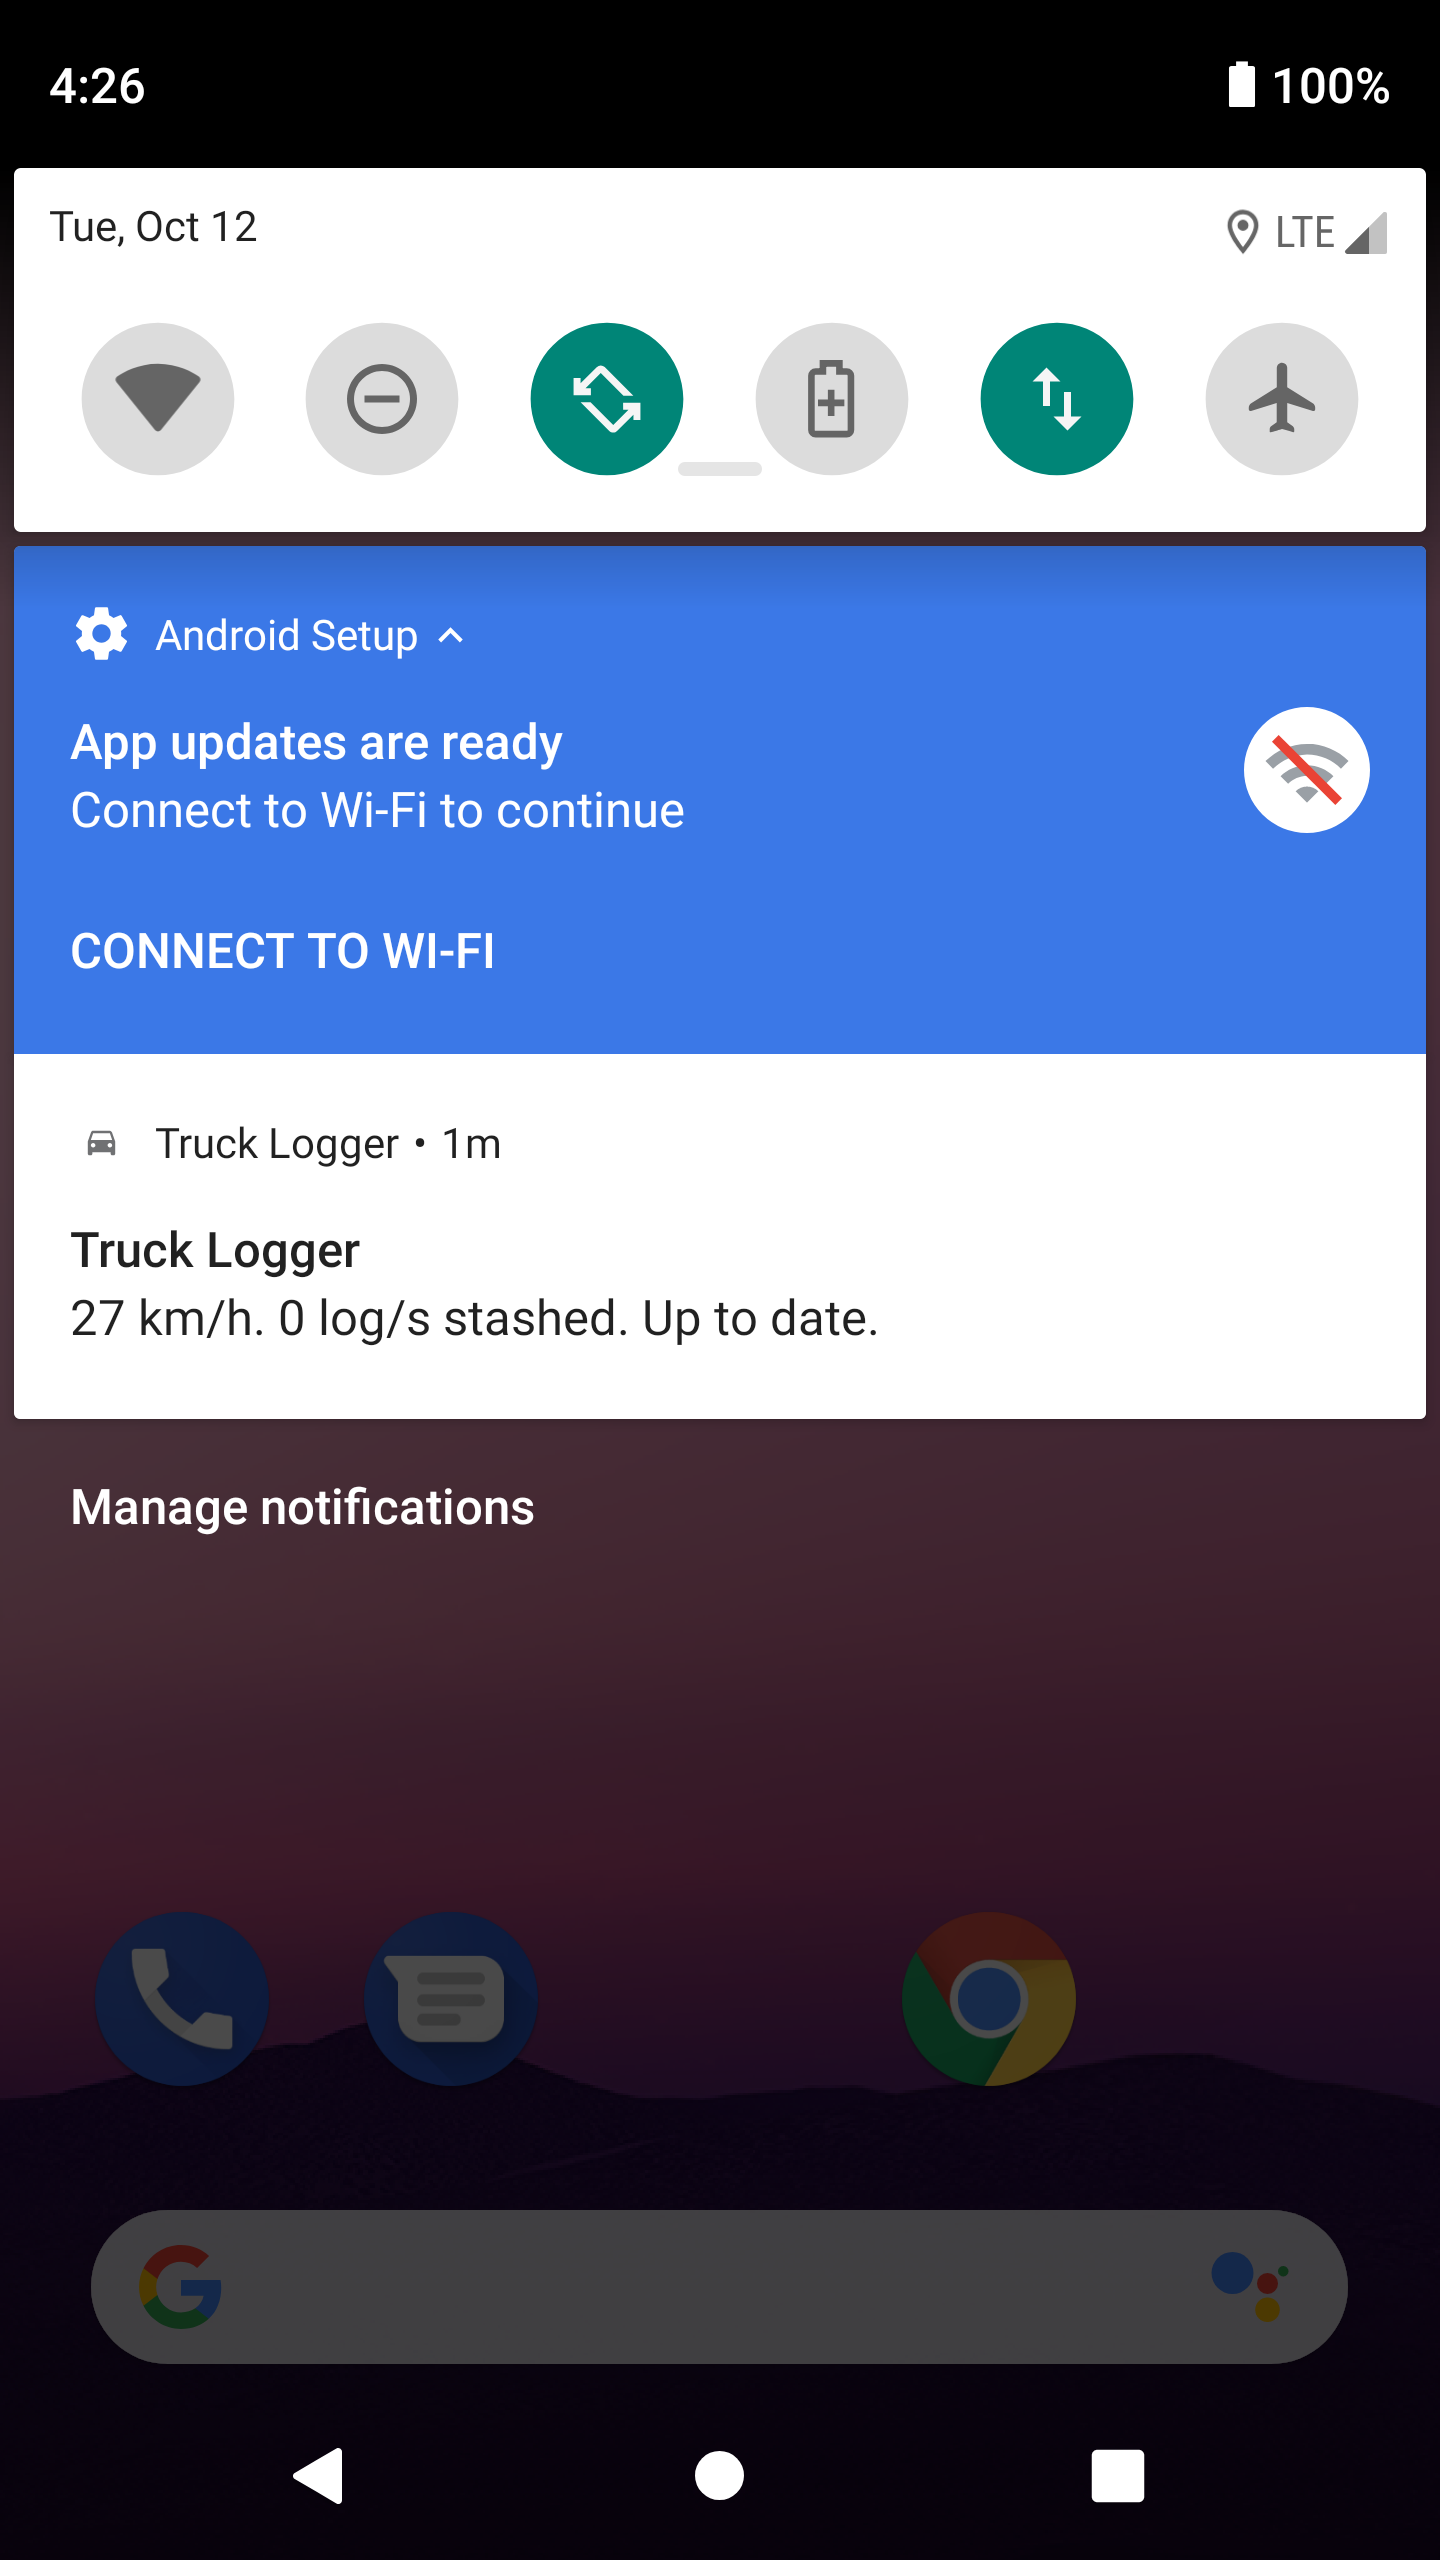
\includegraphics[height=2.5in]{android_app_background.png}
        \label{fig:android_app_background}
    }
    \subfigure[Stashing logs locally]
    {
        \centering
        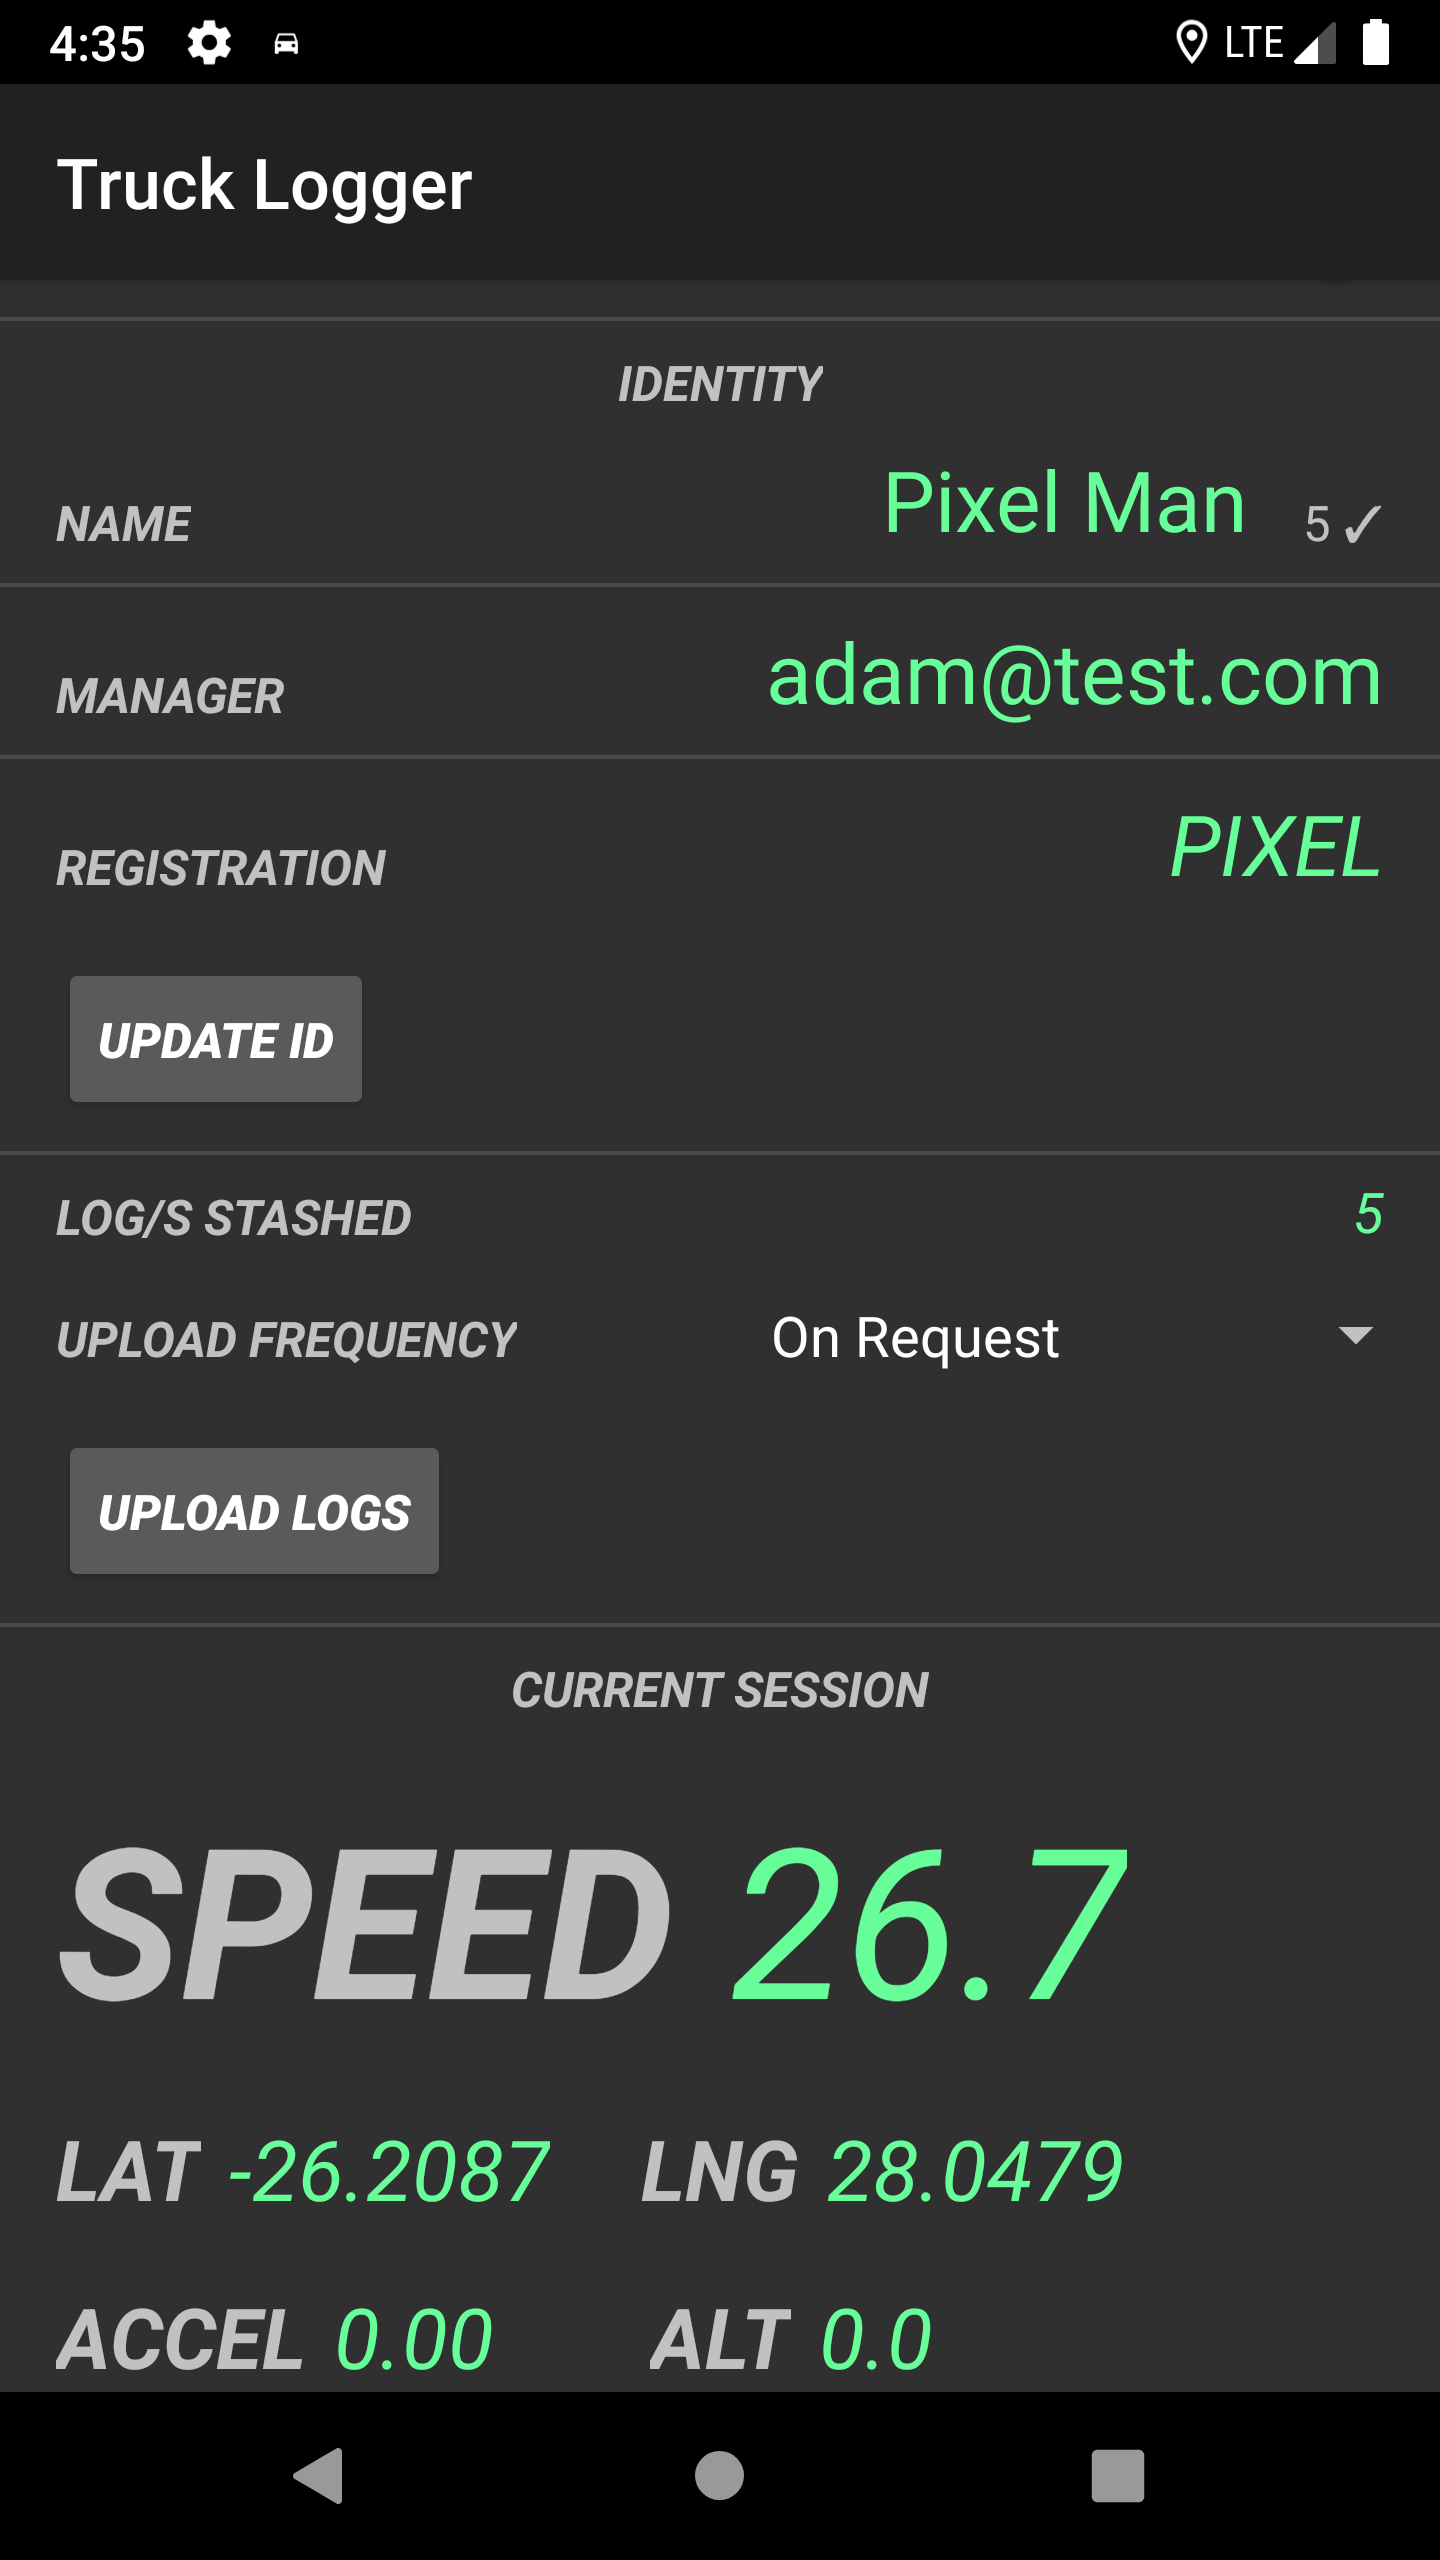
\includegraphics[height=2.5in]{android_app_stashing.png}
        \label{fig:android_app_stashing}
    }
\caption{Android application - Implemented layout}
\label{fig:android_app_implementation}
\end{figure}

The \ac{ui} provides an interface detailing \ac{id} information related to the trucker and manager.
Users can update their \ac{id} as long as they have connectivity to the server.
They can also upload all log data at any instance.

Figure \ref{fig:android_app_idle} depicts the application in an idle state.
The application performs no logging in this state.

Toggling the status check box allows the application to start logging data, as seen in figure \ref{fig:android_app_running}.
This activates the background process which polls for \ac{gps}, acceleration (provided the linear composite accelerometer if available) and altitude.
While tracking, a constant notification is displayed, indicating speed and number of logs stashed.

Depending on the upload frequency, an attempt is made to upload logs to the central server.
Otherwise logs are stashed in the SQLite database.

\subsection{\Ac{io} Server}
Figure \ref{fig:io_output} depicts the output of the \ac{io} server, logging request information from multiple users to standard output.

\begin{figure}[H]
\centering
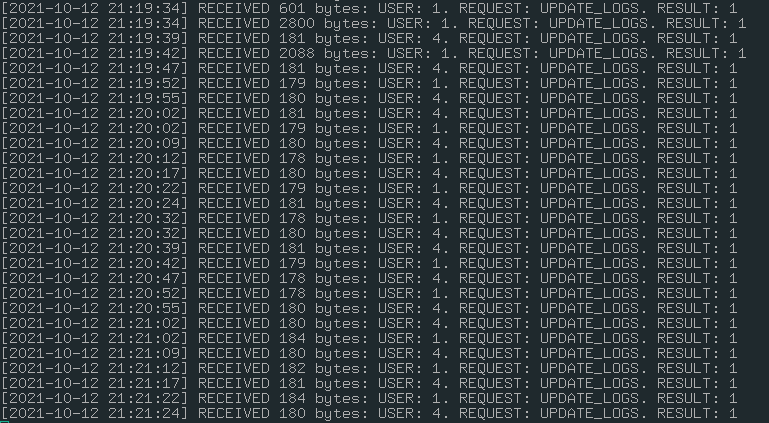
\includegraphics[scale=0.60]{io_output.png}
\caption{IO Server - Request information logged to standard output}
\label{fig:io_output}
\end{figure}

The \Ac{io} server handles \ac{ssl} connections transmitting a serialized \ac{json} payload consisting of the truckers \ac{id}, \ac{uuid} and extra data (detailed in figure \ref{fig:json_protocol}).
The \ac{uuid} is added to ensure that one trucker can be associated with a device.
Depending on the request code provided, the server processes each request appropriately.

\subsubsection{Requests}
The \ac{io} server handles various requests.
Each request type is specified by a request code, as shown in figure \ref{fig:json_protocol}.
\begin{enumerate}
\item \textbf{UPDATE ID}\\
The trucker sends a request to update their \ac{id} with a newly generated \ac{uuid}.
As long as the \textit{Verified} flag is set to false, the server will update its record of the \ac{uuid} corresponding to that trucker \ac{id}.
The manager must first set the flag to false if they need to reset the trucker's device or change the identity associated with a specific trucker.
The \textit{Verified} flag is then set to true.
All future requests must provide the \ac{uuid}.

\item \textbf{VERIFY ID}\\
This request ensures that a truckers \ac{id} and \ac{uuid} correspond in the database.
If not, the server returns a \textit{INVALID CREDENTIALS} response code.
This mechanism ensures that only one device can send logs for a corresponding trucker \ac{id}.

\item \textbf{UPDATE LOGS}\\
This request first performs logic for verifying \ac{id}s, associated with the \textit{VERIFY ID} request.
If the incoming \ac{id} is valid, the log records for the specific device are added to the database.
\end{enumerate}

\subsubsection{Responses}
The server responds with an appropriate response code, to the android requests.
\begin{enumerate}
\item \textbf{FAIL}\\
A fail code indicating the response was invalid.
\item \textbf{OK}\\
A success code indicating the response was valid.
\item \textbf{INVALID CREDENTIALS}\\
A fail code indicating that the client's \ac{id} and \ac{uuid} do not correspond.
\item \textbf{DB CONN FAILED}\\
A server error triggered by an exception when the server can't establish connection with the database.
\item \textbf{PARSE FAIL}\\
The incoming \ac{json} serialized payload was malformed and could not be deserialized.
\end{enumerate}

\subsection{Web application}
The web application is implemented using the \textit{ASP.NET Core} framework, running in Linux on the Kestrel web server.

\subsubsection{User login and signup}
Microsoft's \textit {ASP.NET Core Identity} library provides an easy automated interface for handling manager identity.
It provides user log in and sign up pages, as seen in figure \ref{fig:webapp_userhandling}.

\begin{figure}[H]
\centering
    \subfigure[Sign up]
    {
        \centering
        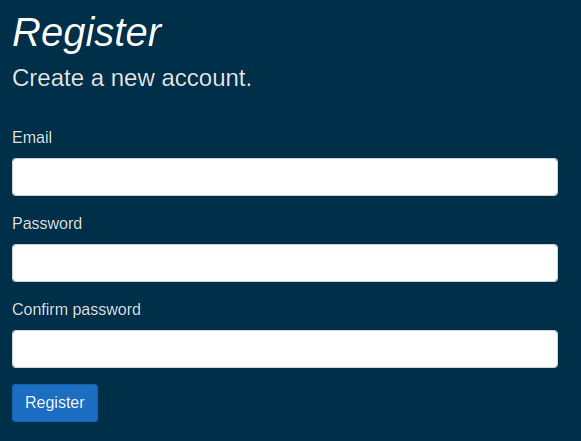
\includegraphics[width=2.5in]{webapp_signup.png}
        \label{fig:webapp_signup}
    }
    \subfigure[Log in]
    {
        \centering
        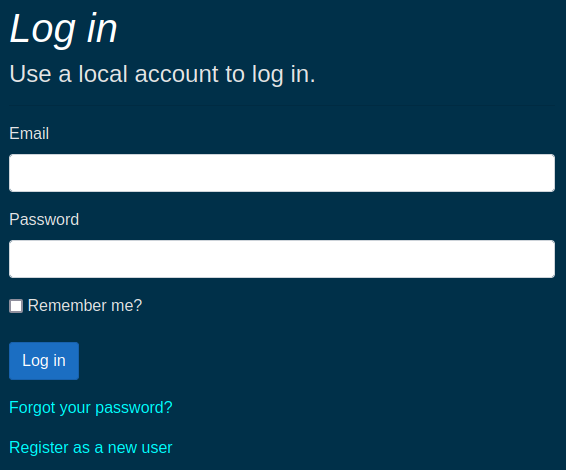
\includegraphics[height=2.5in]{webapp_login.png}
        \label{fig:webapp_login}
    }
\caption{Web application - Manager account handling}
\label{fig:webapp_userhandling}
\end{figure}

\subsubsection{Fleet viewing and management}
The Fleet Controller is implemented in handling \Ac{http} requests for serving web pages related to the manager's Fleet.
Fleet Controller methods are called when the \ac{uri} in the address bar is appended with the text \textit{Fleet}.

\begin{figure}[H]
\centering
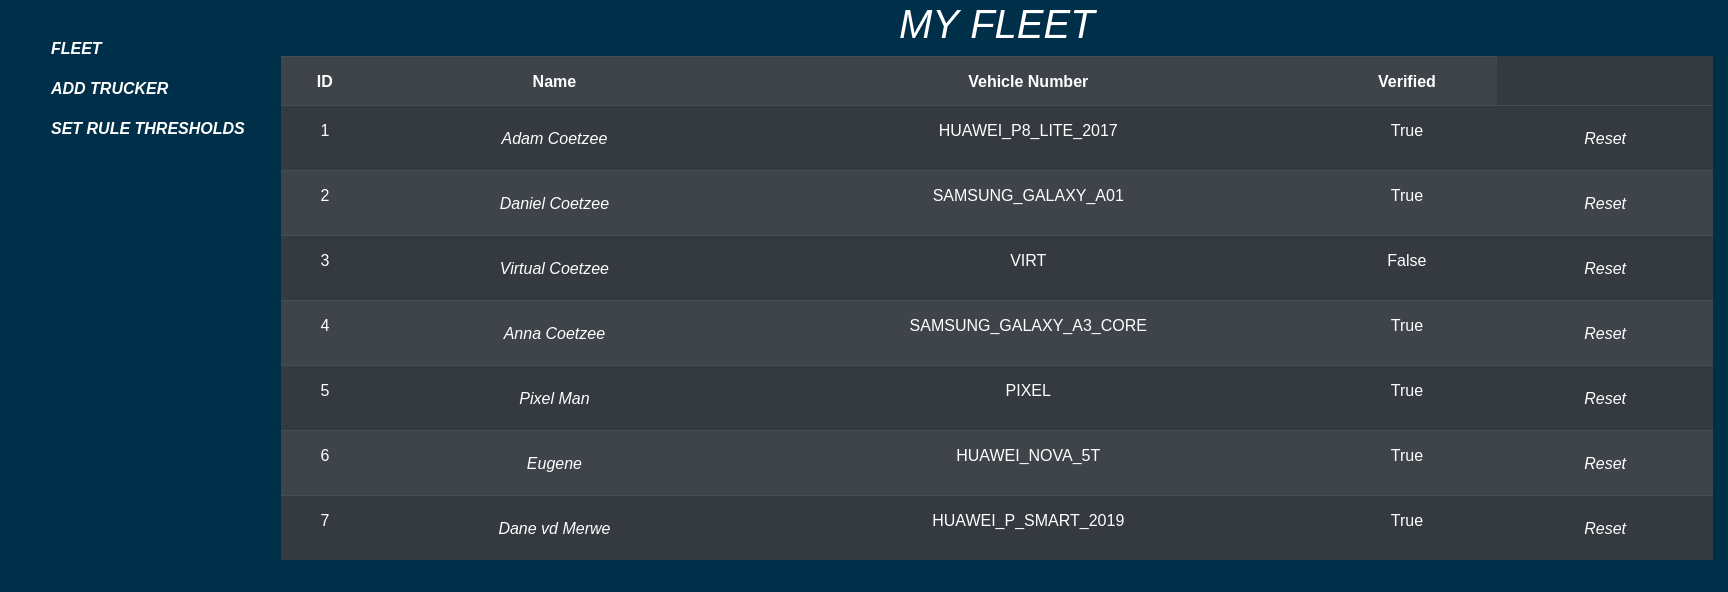
\includegraphics[width=6in]{webapp_fleet_index.png}
\caption{Web application - Fleet Index}
\label{fig:webapp_fleet_index}
\end{figure}
The Fleet Index page shown in figure \ref{fig:webapp_fleet_index} displays a list of all truckers in the manager's fleet.
The \textit{Verified} attribute indicates whether a trucker is paired to a specific device.
This attribute can be reset to allow the pairing process to be performed again for the same or a new device.

\begin{figure}[H]
\centering
    \subfigure[Add Trucker]
    {
        \centering
        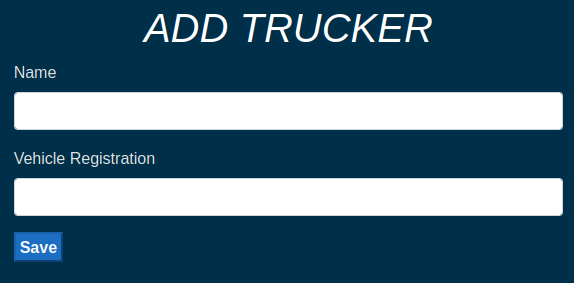
\includegraphics[width=2.5in]{webapp_add_trucker.png}
        \label{fig:webapp_add_trucker}
    }
    \subfigure[Set rules]
    {
        \centering
        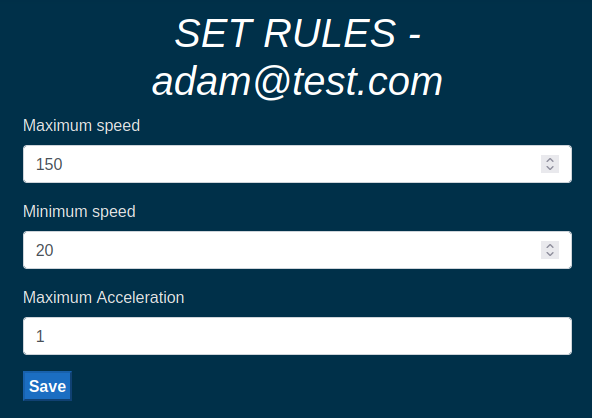
\includegraphics[height=2.5in]{webapp_set_rules.png}
        \label{fig:webapp_set_rules}
    }
\caption{Web application - Fleet management}
\label{fig:webapp_fleet_management}
\end{figure}
Figure \ref{fig:webapp_fleet_management} depicts pages implemented for adding truckers and setting rule thresholds.
They both make use of \ac{html} forms bound to the Manager and Trucker model.
\Ac{http} requests are routed to the Fleet Controller and handled by an appropriate method.

\subsubsection{Trucker activity}
\begin{figure}
\centering
    \subfigure[View Trucker]
    {
        \centering
        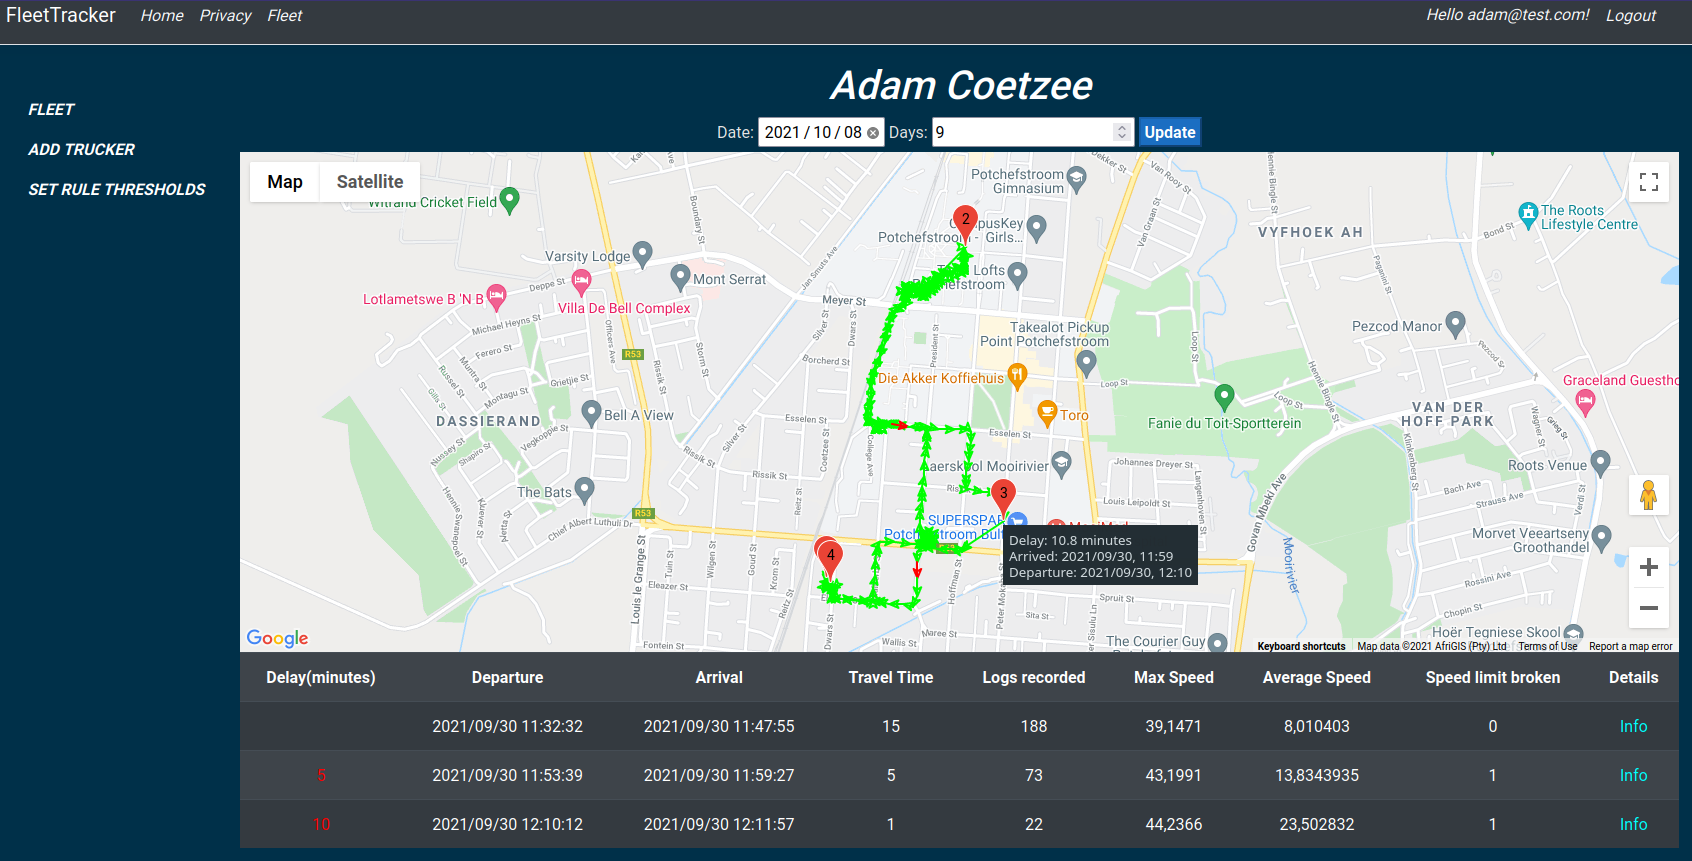
\includegraphics[width=6in]{webapp_view_trucker.png}
        \label{fig:webapp_view_trucker}
    }
    \subfigure[View Trip]
    {
        \centering
        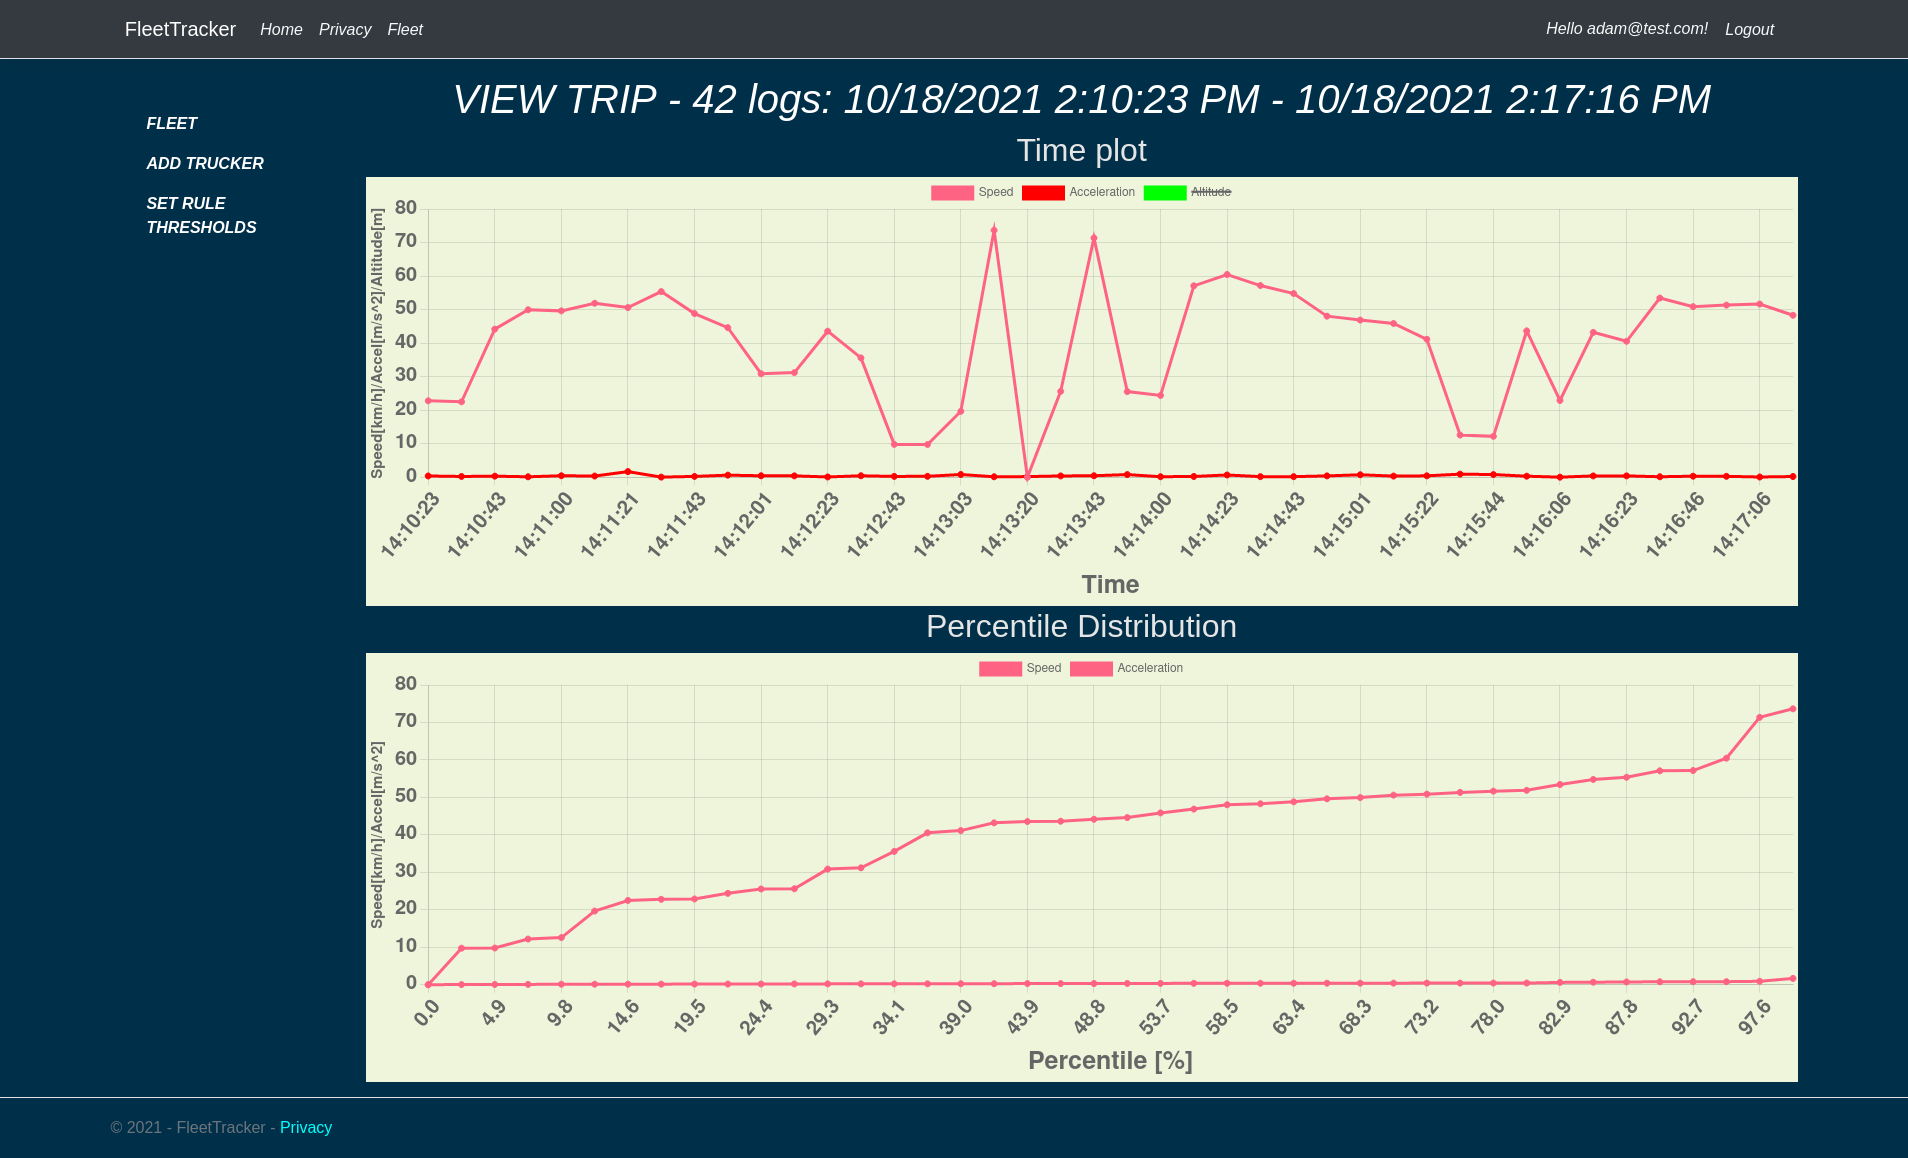
\includegraphics[width=6in]{webapp_view_trip.png}
        \label{fig:webapp_view_trip}
    }
\caption{Web application - Trip collection and information}
\label{fig:webapp_trucker_details}
\end{figure}
Figure \ref{fig:webapp_trucker_details} details the interface for viewing trucker activity.

Figure \ref{fig:webapp_view_trucker} provides a time adjustable page which groups the logs into individual trips.
A map is rendered (using the Google JavaScript \Ac{api}) with routes physically drawn in the map, using arrows.
If the defined speed limit is broken, the arrows are drawn in red.
Stopping points are indicated with markers labeled in chronological order.
Hovering over a stop label indicates how long the trucker had stopped at a given location.
A table is rendered displaying this information.

Figure \ref{fig:webapp_view_trip} allows a more detailed view of an individual trip between two markers.
Time plots indicate give speed, acceleration and altitude plots which vary with time as truckers carry out their trips.
A percentile plot is included to visualize the spread of speed and acceleration.
This allows managers to visualize what portions of the trip was driven with specific behavior.

\subsection{Deployment}
The web application and \ac{io} server are deployed to a Linux \ac{vps} with access to a static \ac{ip} address and domain name.
A non-profit \ac{ca} Lets Encrypt provides \ac{ssl} certificates, which are required for Android applications which make use \ac{ssl} communication.

Docker containers are created and used for used for deploying the MySQL database and \ac{io} server. 
They are useful for managing dependencies and preventing unwanted changes to the host server.

A link is provided for downloading the Android application as an \ac{apk} file.

\pagebreak

\section{Evaluation}
Evaluation of the system is performed by testing the deployed \ac{io} server and web application with several Android devices which are available.

\begin{table}[H]
\caption{Android devices tested}
\label{tab:android_devices_tested}
\begin{tabular}{llll}
\hline
Android Device      & Price[R]  & Major Android Version & Linear Accelerometer \\ \hline
Huawei P8 Lite 2017 & 2900     & 8                     & Yes                  \\
Samsung Galaxy A01  & 2180     & 10                    & No                   \\
Galaxy A3 Core      & 1400     & 10                    & No                   \\
Huawei Nova 5T      & 7700     & 10                    & Yes                  \\ \hline
\end{tabular}
\end{table}

\subsection{Location accuracy}
Generally, \ac{gps} accuracy is reasonable, within an approximately 20 meter range.
Occasionally, a rogue data point occurs resulting in a random spike, as shown in figure \ref{fig:random_spike}.
A small adjustment is made to algorithm \ref{algo_agg}, where the proceeding log is also compared with the current log in each iteration of the for loop.
This ensures that two consecutive logs must be greater than the distance threshold, when aggregating nearby data points.
The result of this correction is depicted in figure \ref{fig:random_spike_correct}.

\begin{figure}[H]
\centering
    \subfigure[Random spike]
    {
        \centering
        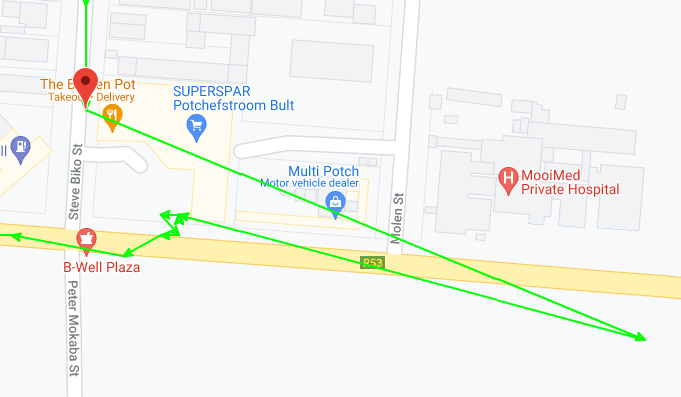
\includegraphics[width=2.5in]{random_spike.png}
        \label{fig:random_spike}
    }
    \subfigure[Correction]
    {
        \centering
        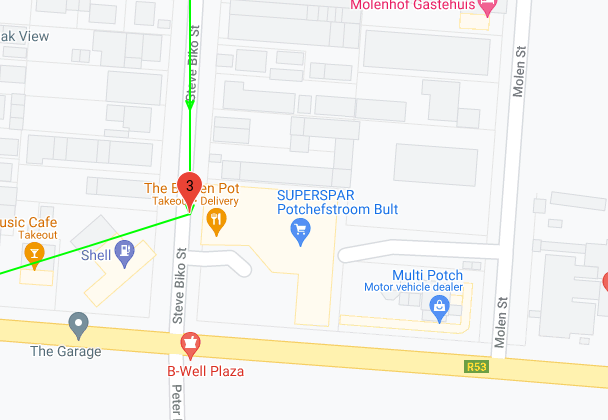
\includegraphics[width=2.5in]{random_spike_correct.png}
        \label{fig:random_spike_correct}
    }
\caption{Location spike correction}
\label{fig:spike_correction}
\end{figure}

\begin{figure}[H]
\centering
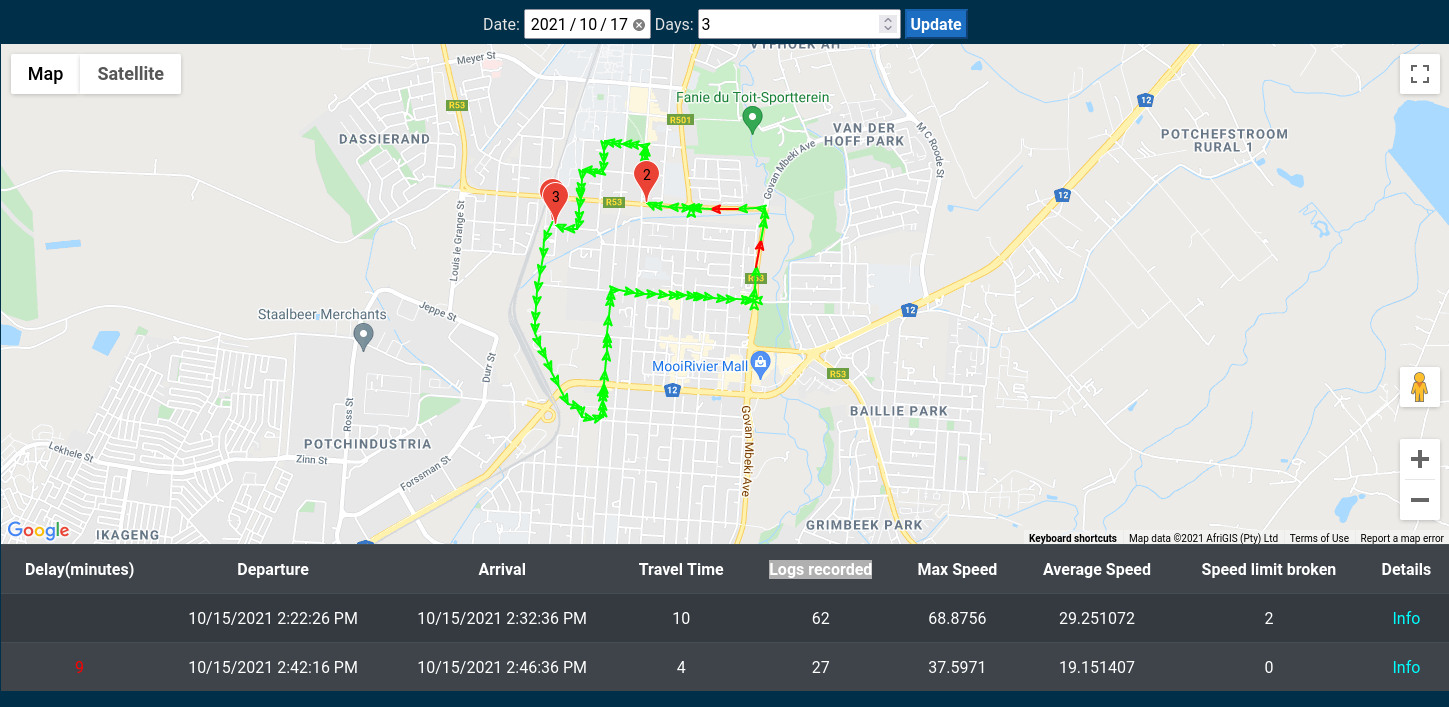
\includegraphics[width=6in]{eval_location.png}
\caption{Location Tracking with the A3 Core}
\label{fig:eval_location}
\end{figure}

The four devices are taken on the same trip through town, with the logging frequency set to 10 seconds.
They all register near identical arrival and departure times, and sketch the same route on the map, as depicted in figure \ref{fig:eval_location}.
With the speed limit set to 60km/h, portions of the trip were correctly logged above this speed.
Other statistics all indicate similar trends.

\begin{figure}[H]
\centering
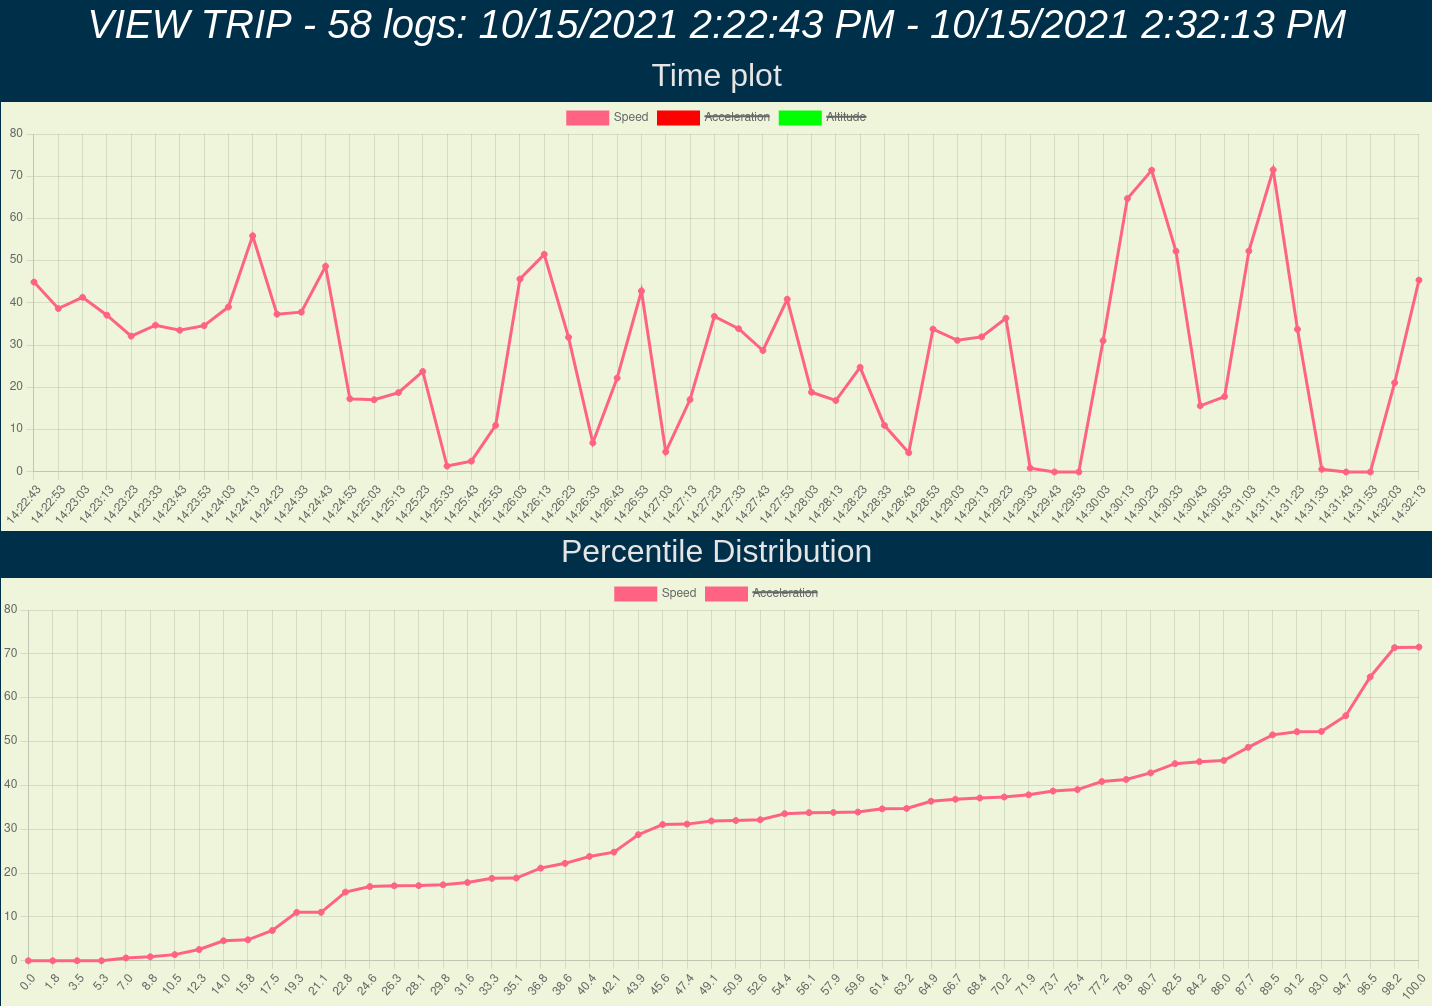
\includegraphics[width=5in]{eval_speed.png}
\caption{Speed data}
\label{fig:eval_speed}
\end{figure}

\begin{figure}[H]
\centering
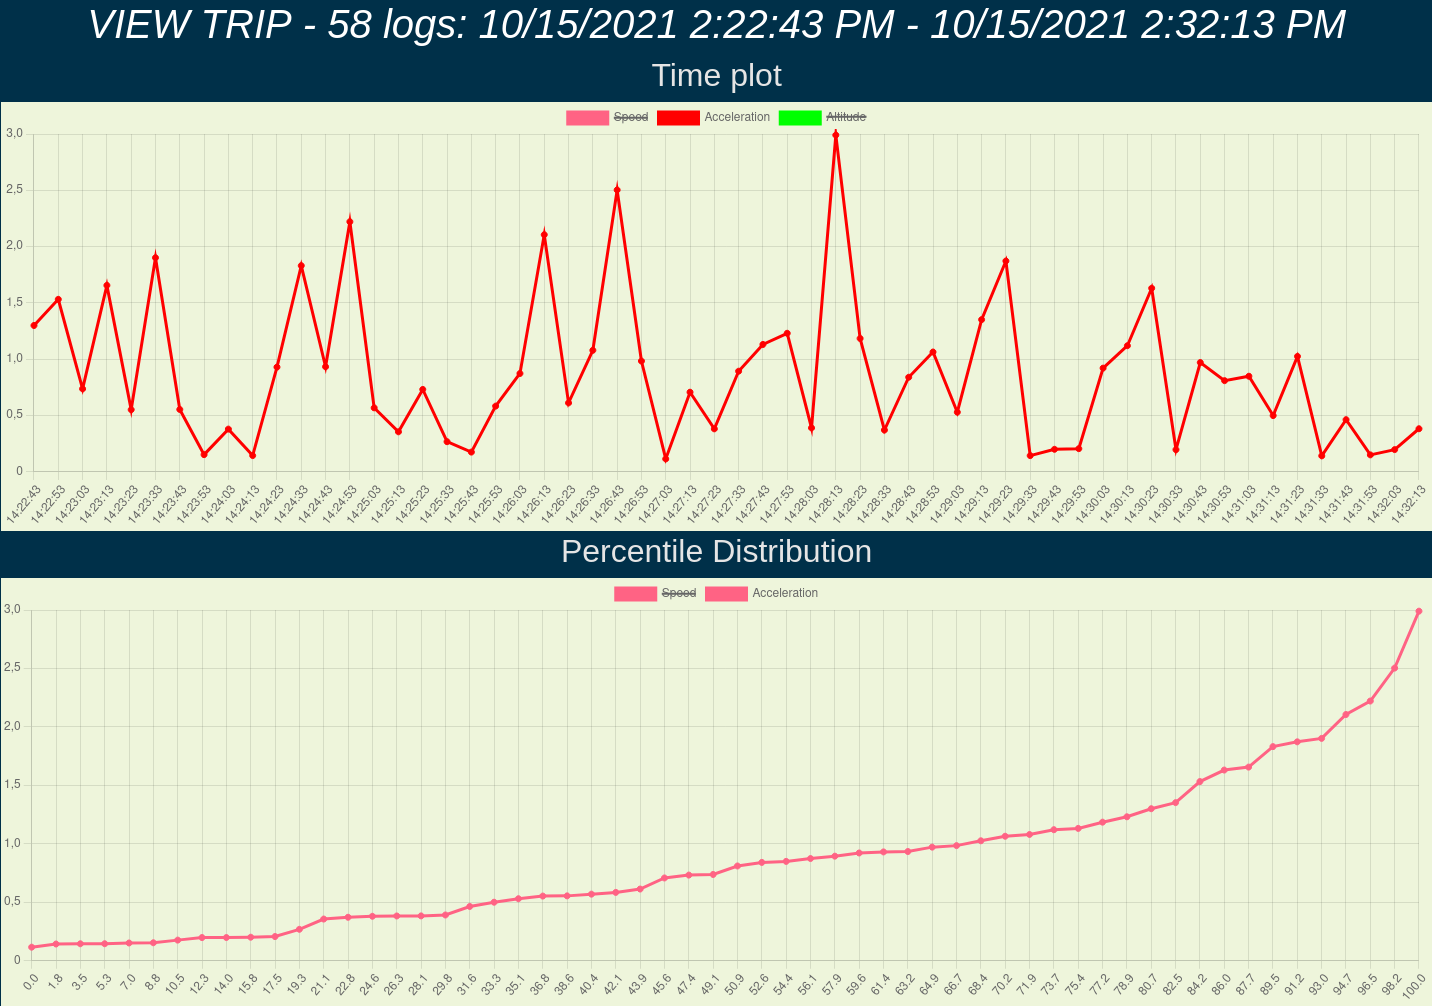
\includegraphics[width=5in]{eval_accel.png}
\caption{Acceleration Data}
\label{fig:eval_accel}
\end{figure}

\begin{figure}[H]
\centering
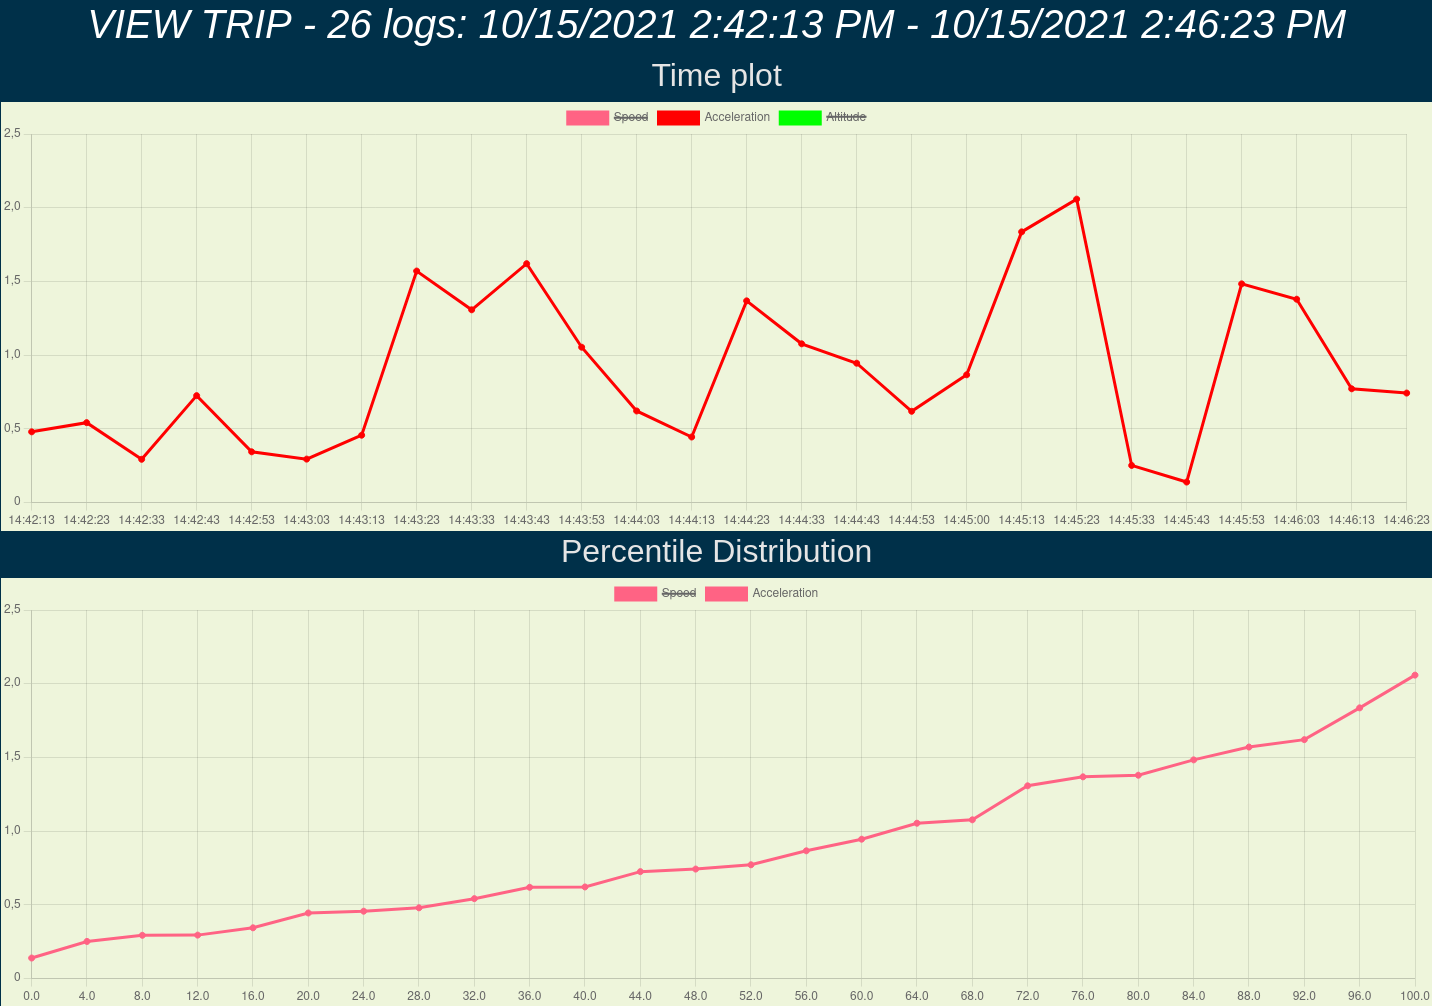
\includegraphics[width=5in]{eval_accel_slow.png}
\caption{Acceleration Data - Slow}
\label{fig:eval_accel_slow}
\end{figure}

\begin{figure}[H]
\centering
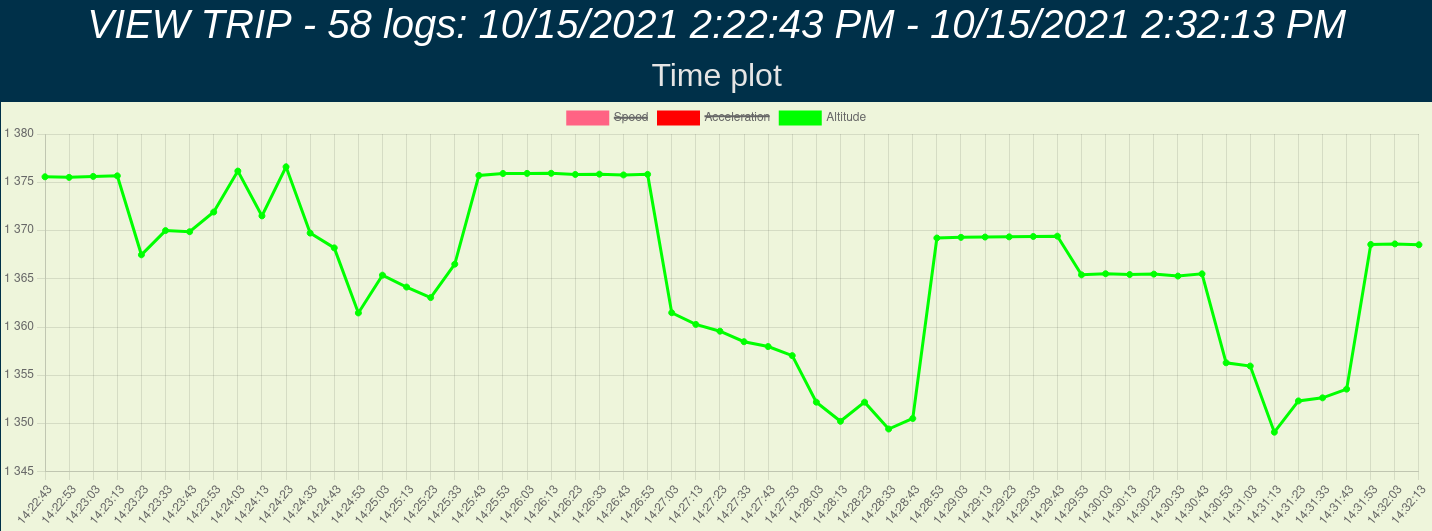
\includegraphics[width=5in]{eval_altitude.png}
\caption{Altitude Data}
\label{fig:eval_altitude}
\end{figure}

\subsection{Android application}
Four Android devices were readily available for testing purposes, which are highlighted in table \ref{tab:android_devices_tested}.

\subsubsection{Application reliability}
Application reliability is tested by ensuring that the tracking service remains active indefinitely.
It is noted that on the Huawei P8 Lite 2017 (running Android 8), the service crashes and stops logging every few hours.
Checking Android debug logs revealed little as to the cause of this crash.

All devices running Android 10 run indefinitely without issue.

\subsubsection{Application Profiling}
The application is profiled in the Android Studio, generating plots for \ac{cpu}, \ac{ram} and network usage as shown in figure \ref{fig:android_profiling}.
\begin{figure}[H]
\centering
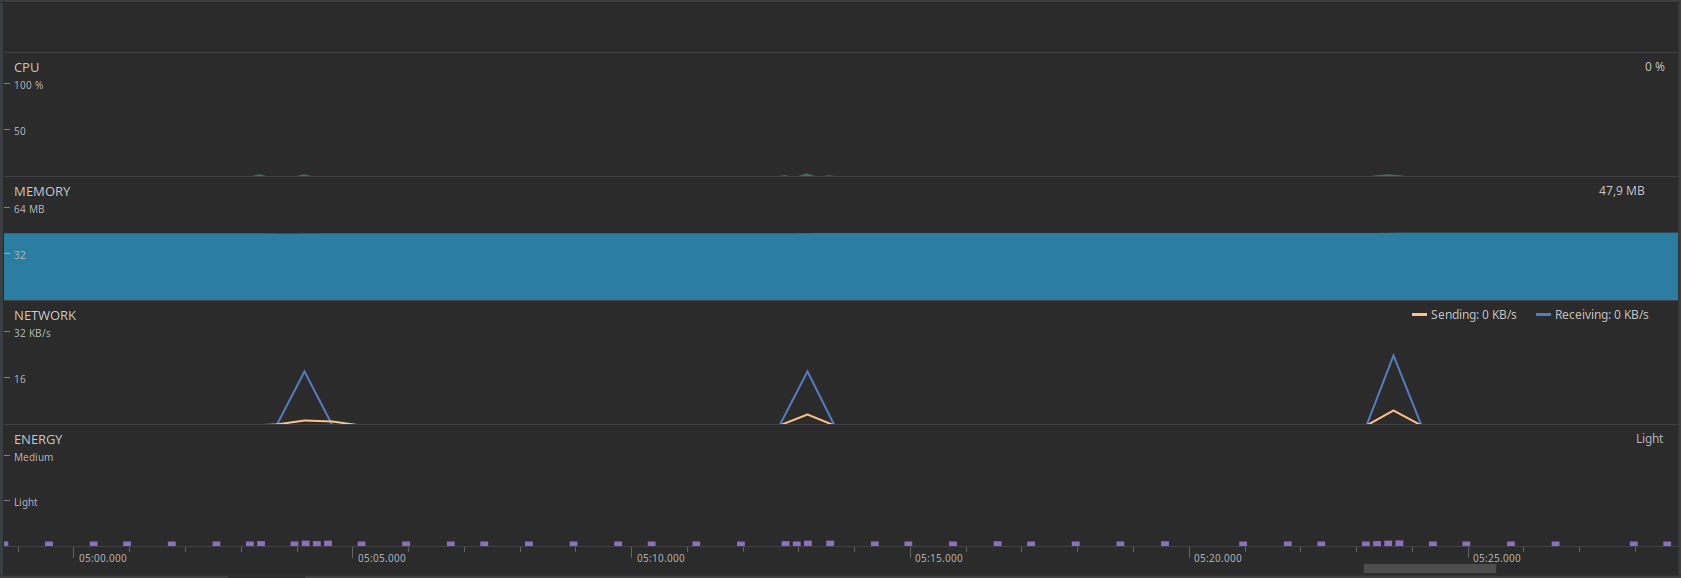
\includegraphics[width=6in]{android_profiling.png}
\caption{Android Profiling}
\label{fig:android_profiling}
\end{figure}
It is noted that the application runs relatively lightly on the system, consuming minimal power and \ac{cpu}.
Typically only 50MB of \ac{ram} is utilized by the application.

\begin{figure}[H]
\centering
    \subfigure[Data Usage]
    {
        \centering
        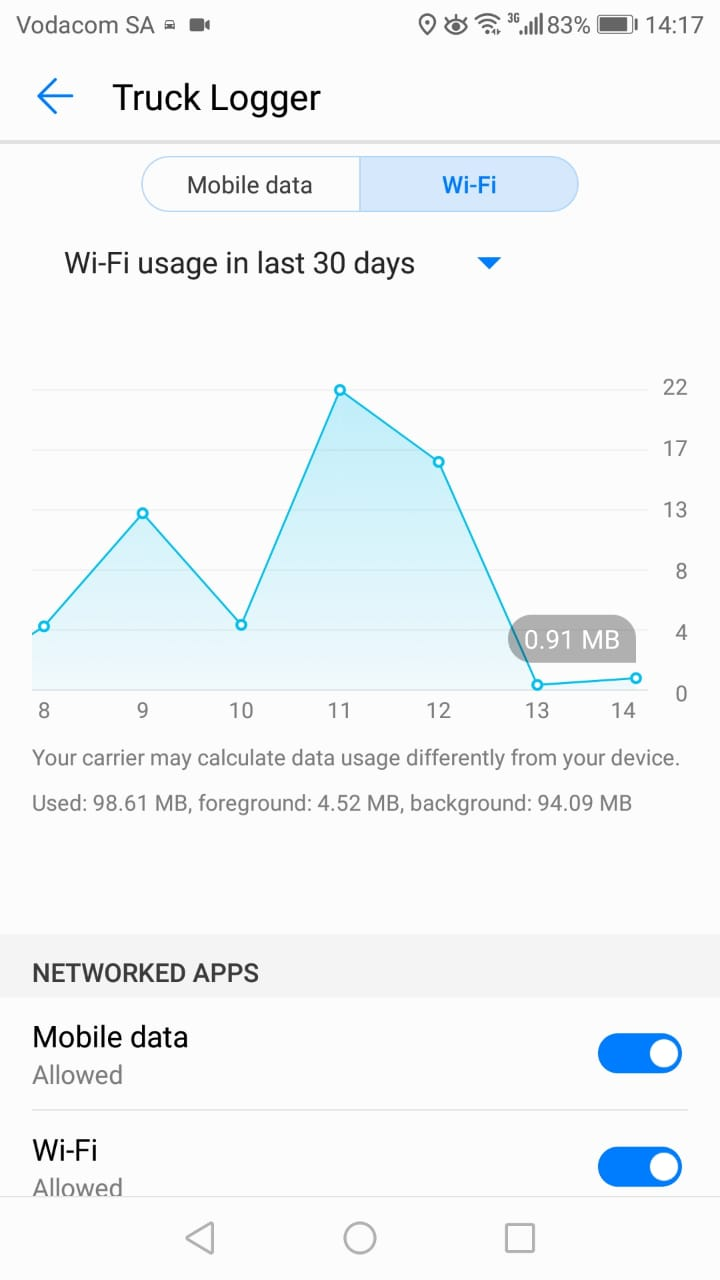
\includegraphics[height=2.5in]{android_data_usage.jpeg}
        \label{fig:android_data_usage}
    }
    \subfigure[Up Time]
    {
        \centering
        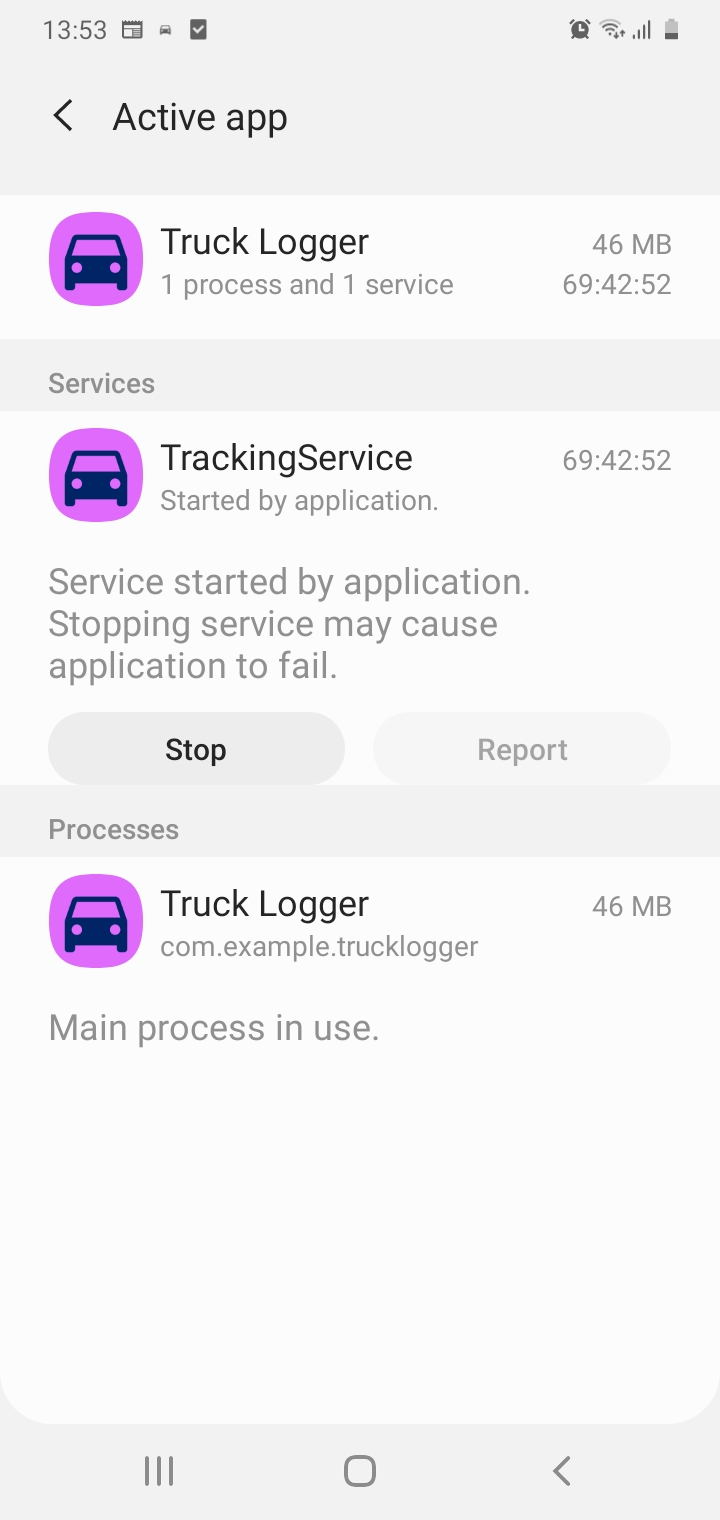
\includegraphics[height=2.5in]{android_app_uptime.jpeg}
        \label{fig:android_app_uptime}
    }
\caption{Android application - up time and data usage}
\label{fig:performance}
\end{figure}

Figure \ref{fig:android_data_usage} details monthly data usage during development on the Huawei P8 Lite 2017, during which the application was logging at a 5 second interval.
In this time, the application consumed approximately 100MB of data.

Figure \ref{fig:android_app_uptime} details the up-time of the application on the Galaxy A3 Core.
The application is seen achieving uninterrupted up-time of approximately 70 hours.

\subsection{\Ac{io} server and web application}
Due to proper exception handling, both the \ac{io} server and web application remain online indefinitely.
Any exceptions that occur with parsing data are properly handled, without compromising data.

\pagebreak

\section{Conclusion}
In this project, a trucker tracking solution is proposed, designed and implemented using log data generated by Android smartphones. 
The log data containing acceleration, altitude, location and speed is stored in a central server and made available to managers for monitoring.
The data is processed to generate useful summaries indicating the trucker's movement and driving behavior.

\subsection{Meeting objectives, requirements and deliverables}
The implemented solution meets the primary objective, by providing detailed reports about the truckers whereabouts.
Managers can view (both visually on a map and in a tabulated form) where the truckers have been.
Managers can also view acceleration, altitude and speed data for trips executed by truckers with reasonable precision.

Technical requirements and deliverables are achieved.
The Android application runs in the background and logs data in the required interval.
Logging data can be uploaded at a predefined frequency or on request.

The \ac{io} server and web application are reliable and run indefinitely.
An intuitive user interface is provided to managers for the purposes of managing and viewing their fleets.

\subsection{Usability}
In a deployment environment, managers will have to ensure that truckers using the android application do so diligently and restart the service if the device shuts down (or in the case of an occasional crash).

The Android application appears to perform more reliably on newer Android versions.
For minimal cost the Samsung Galaxy A01 offers a popular option.

Battery life of Android devices is slightly reduced when running the application, although most devices should be able to adequately perform for 8 hours.
It would be recommended that truckers make use of chargers while en route.

\subsection{Future Improvements}
A few aspects are considered in improving the system for commercial applications.

\subsubsection{External sensor integration}
Trucks which make use of the \ac{can} protocol can be interfaced with additional hardware to give more detailed information about trucks.
This includes data such as wheel speed, fuel and oil readings among others.
Such an addition will allow managers better monitoring of their vehicles, allowing for preventative maintenance.

\subsubsection{Improving the robustness of the Android application}
If the android application stops running, or the device restarts, it requires manual intervention by the trucker to restart the service.
It would be beneficial to implement the automatic startup of the application upon crashing or booting the device.

\subsubsection{Serialization protocol and data usage}
The \ac{json} protocol used for communication contains an element of redundant data which makes it more debuggable at the expense of data usage.
This is due to the repetition of key text used to identify the corresponding value associated with the key.
Serialization libraries such as Google's Protobuf library offer room for improvement.

The current implementation opens and closes sockets with every connection.
This is undesirable due to the significant data usage overhead associated with establishing encrypted \ac{ssl} connections.
It would be desirable to rather keep socket connections open.

\subsubsection{Sensor fusion}
Speed in the implemented solution is determined by taking consecutive \ac{gps} readings and comparing them with the time elapsed.
While adequate for straight paths, speed accuracy for larger sampling intervals is reduced especially for curved paths.

More intelligent use of on-board sensors (sensor fusion) has potential to more accurately infer speed and location.
This would increase the logging accuracy.

\subsubsection{Accelerometer data}
Logging accelerometer data periodically offers limited insight into the driving behavior of truckers, as large time periods where truckers could be misbehaving, are neglected.
A smoother mechanism would be required, making use of continuous polling.

\subsection{Conclusion}
The truck tracking system is realized to meet the primary objectives, goals and deliverables.
Software engineering methods and practices are utilized in the design, development and implementation of the system.

While the system developed offers insight into the whereabouts of truckers, there is potential for more driver-specific behavior to be inferred.

The system requires some improvement in robustness, to be deployed in commercial applications.


\pagebreak

\bibliographystyle{IEEEtran}
\bibliography{ref.bib}
\pagebreak

\appendices

\section{Low-level implementation Details}\label{uml}
\subsection{Android Application}\label{App:android}
\begin{figure}[H]
\centering
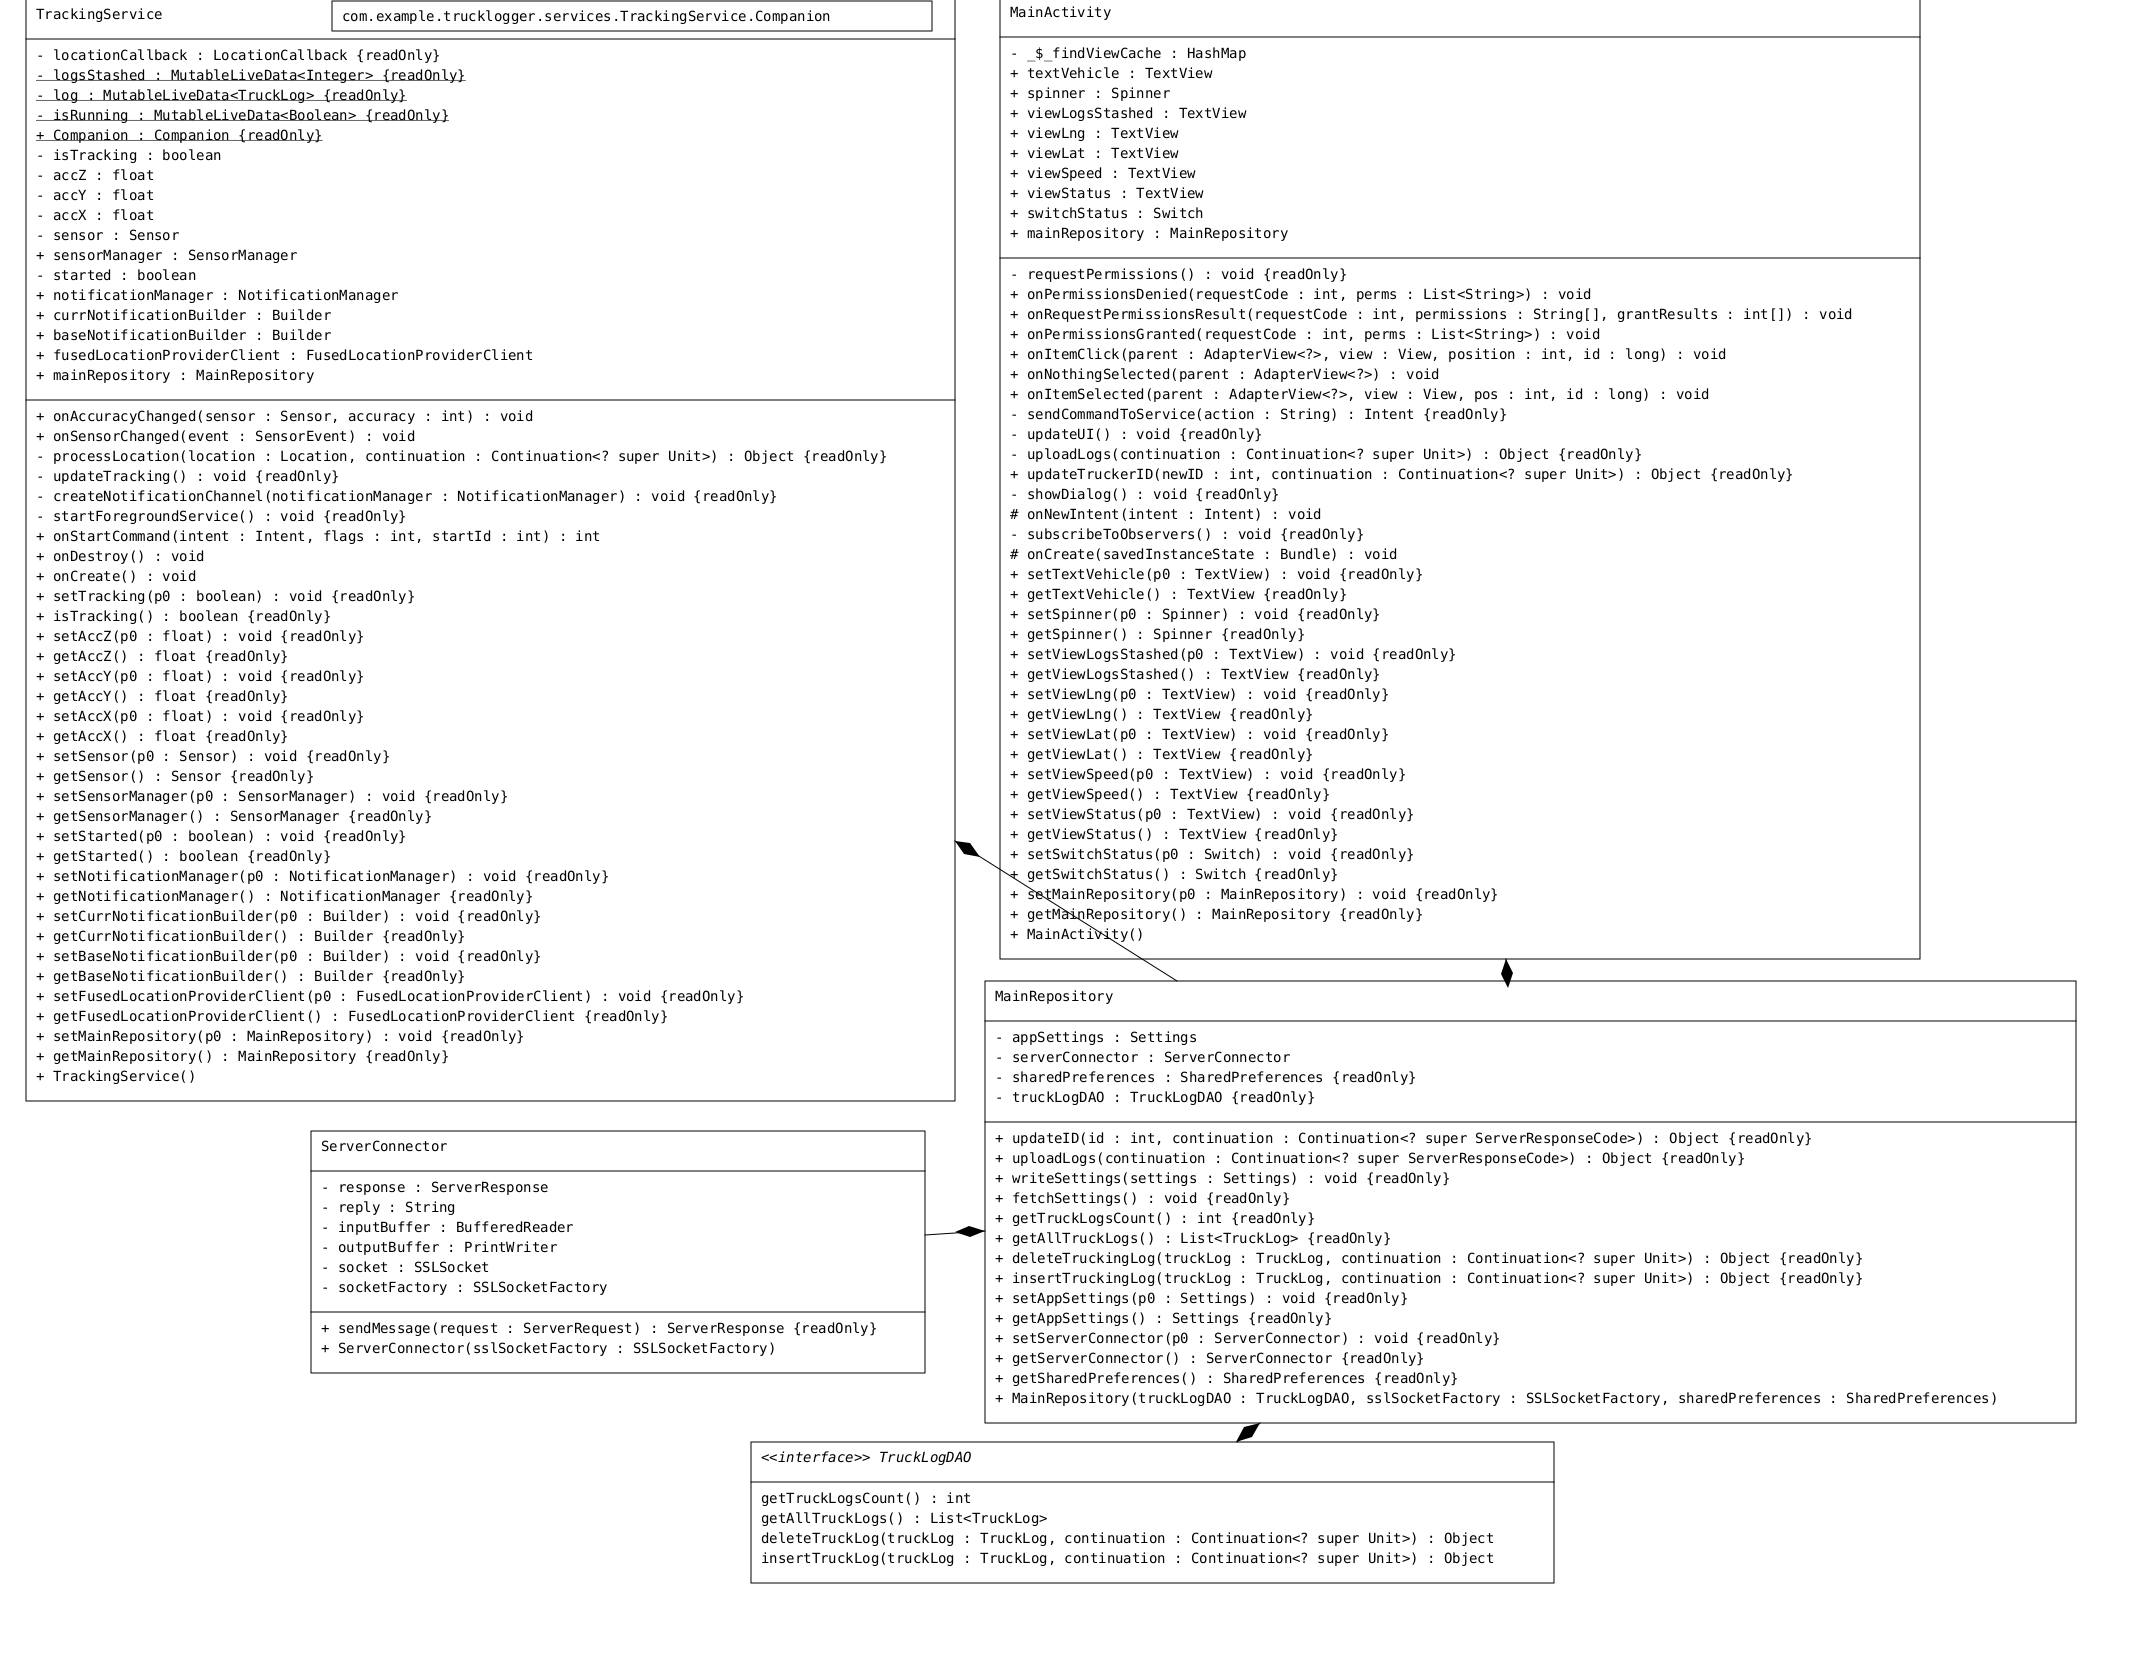
\includegraphics[width=6.5in]{uml_android.png}
\caption{Android Application - Abridged \ac{uml} diagram}
\label{fig:uml_android}
\end{figure}

Figure \ref{fig:uml_android} depicts an abridged generated \ac{uml} diagram of the android source code.
Much detail is omitted for the sake of simplicity.
It is noted that much of the initially planned architecture is successfully implemented.
\pagebreak

\subsection{\ac{io} Server}\label{App:io_server}
\begin{figure}[H]
\centering
    \subfigure[Server]
    {
        \centering
        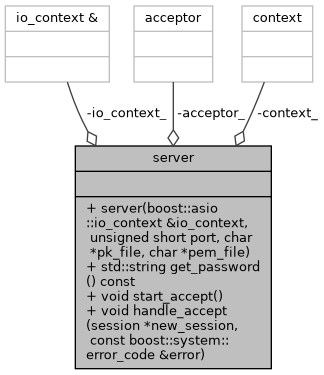
\includegraphics[height=3in]{../diag/io_server.png}
        \label{fig:io_server}
    }
    \subfigure[Session]
    {
        \centering
        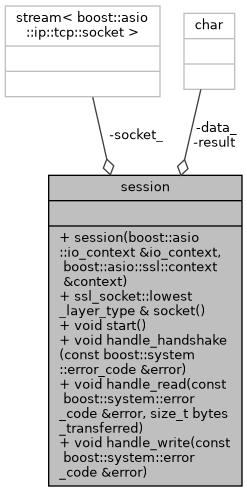
\includegraphics[height=3in]{../diag/io_session.png}
        \label{fig:io_session}
    }\\
    \subfigure[Handler]
    {
        \centering
        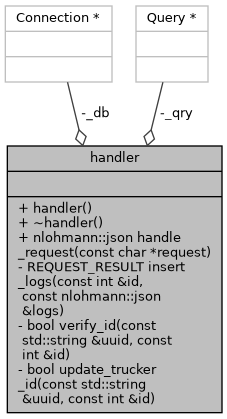
\includegraphics[height=3in]{../diag/io_handler.png}
        \label{fig:io_handler}
    }
\caption{\ac{io} Server - Classes}
\label{fig:uml_io}
\end{figure}

\begin{figure}
\centering
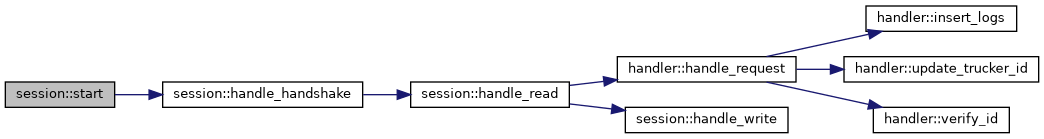
\includegraphics[width=6in]{io_flow.png}
\caption{\ac{io} Server - Functional Flow}
\label{fig:io_flow}
\end{figure}

Figure \ref{fig:uml_io} depicts the class methods implemented in the \ac{io} server.
The server class in figure \ref{fig:io_server} details the server implementation, which assigns a session to an incoming connection.
The session class in figure \ref{fig:io_session} handles the verification procedure required for \ac{ssl}, which includes the handshake, encryption and decryption.
The handler class in figure \ref{fig:io_handler} handles the actual implemented business logic required for operation, including verification, updating \ac{id}s and inserting new log data.

The typical flow (method calling order) of each connection is detailed in \ref{fig:io_flow}.

\end{document}
